
%% bare_jrnl.tex
%% V1.4b
%% 2015/08/26
%% by Michael Shell
%% see http://www.michaelshell.org/
%% for current contact information.
%%
%% This is a skeleton file demonstrating the use of IEEEtran.cls
%% (requires IEEEtran.cls version 1.8b or later) with an IEEE
%% journal paper.
%%
%% Support sites:
%% http://www.michaelshell.org/tex/ieeetran/
%% http://www.ctan.org/pkg/ieeetran
%% and
%% http://www.ieee.org/

%%*************************************************************************
%% Legal Notice:
%% This code is offered as-is without any warranty either expressed or
%% implied; without even the implied warranty of MERCHANTABILITY or
%% FITNESS FOR A PARTICULAR PURPOSE! 
%% User assumes all risk.
%% In no event shall the IEEE or any contributor to this code be liable for
%% any damages or losses, including, but not limited to, incidental,
%% consequential, or any other damages, resulting from the use or misuse
%% of any information contained here.
%%
%% All comments are the opinions of their respective authors and are not
%% necessarily endorsed by the IEEE.
%%
%% This work is distributed under the LaTeX Project Public License (LPPL)
%% ( http://www.latex-project.org/ ) version 1.3, and may be freely used,
%% distributed and modified. A copy of the LPPL, version 1.3, is included
%% in the base LaTeX documentation of all distributions of LaTeX released
%% 2003/12/01 or later.
%% Retain all contribution notices and credits.
%% ** Modified files should be clearly indicated as such, including  **
%% ** renaming them and changing author support contact information. **
%%*************************************************************************


% *** Authors should verify (and, if needed, correct) their LaTeX system  ***
% *** with the testflow diagnostic prior to trusting their LaTeX platform ***
% *** with production work. The IEEE's font choices and paper sizes can   ***
% *** trigger bugs that do not appear when using other class files.       ***                          ***
% The testflow support page is at:
% http://www.michaelshell.org/tex/testflow/



\documentclass[journal]{IEEEtran}
%
% If IEEEtran.cls has not been installed into the LaTeX system files,
% manually specify the path to it like:
% \documentclass[journal]{../sty/IEEEtran}





% Some very useful LaTeX packages include:
% (uncomment the ones you want to load)


% *** MISC UTILITY PACKAGES ***
%
%\usepackage{ifpdf}
% Heiko Oberdiek's ifpdf.sty is very useful if you need conditional
% compilation based on whether the output is pdf or dvi.
% usage:
% \ifpdf
%   % pdf code
% \else
%   % dvi code
% \fi
% The latest version of ifpdf.sty can be obtained from:
% http://www.ctan.org/pkg/ifpdf
% Also, note that IEEEtran.cls V1.7 and later provides a builtin
% \ifCLASSINFOpdf conditional that works the same way.
% When switching from latex to pdflatex and vice-versa, the compiler may
% have to be run twice to clear warning/error messages.






% *** CITATION PACKAGES ***
%
%\usepackage{cite}
% cite.sty was written by Donald Arseneau
% V1.6 and later of IEEEtran pre-defines the format of the cite.sty package
% \cite{} output to follow that of the IEEE. Loading the cite package will
% result in citation numbers being automatically sorted and properly
% "compressed/ranged". e.g., [1], [9], [2], [7], [5], [6] without using
% cite.sty will become [1], [2], [5]--[7], [9] using cite.sty. cite.sty's
% \cite will automatically add leading space, if needed. Use cite.sty's
% noadjust option (cite.sty V3.8 and later) if you want to turn this off
% such as if a citation ever needs to be enclosed in parenthesis.
% cite.sty is already installed on most LaTeX systems. Be sure and use
% version 5.0 (2009-03-20) and later if using hyperref.sty.
% The latest version can be obtained at:
% http://www.ctan.org/pkg/cite
% The documentation is contained in the cite.sty file itself.






% *** GRAPHICS RELATED PACKAGES ***
%
\ifCLASSINFOpdf
 \usepackage[pdftex]{graphicx}
  % declare the path(s) where your graphic files are
  % \graphicspath{{../pdf/}{../jpeg/}}
  % and their extensions so you won't have to specify these with
  % every instance of \includegraphics
  % \DeclareGraphicsExtensions{.pdf,.jpeg,.png}
\else
  % or other class option (dvipsone, dvipdf, if not using dvips). graphicx
  % will default to the driver specified in the system graphics.cfg if no
  % driver is specified.
  % \usepackage[dvips]{graphicx}
  % declare the path(s) where your graphic files are
  % \graphicspath{{../eps/}}
  % and their extensions so you won't have to specify these with
  % every instance of \includegraphics
  % \DeclareGraphicsExtensions{.eps}
\fi
% graphicx was written by David Carlisle and Sebastian Rahtz. It is
% required if you want graphics, photos, etc. graphicx.sty is already
% installed on most LaTeX systems. The latest version and documentation
% can be obtained at: 
% http://www.ctan.org/pkg/graphicx
% Another good source of documentation is "Using Imported Graphics in
% LaTeX2e" by Keith Reckdahl which can be found at:
% http://www.ctan.org/pkg/epslatex
%
% latex, and pdflatex in dvi mode, support graphics in encapsulated
% postscript (.eps) format. pdflatex in pdf mode supports graphics
% in .pdf, .jpeg, .png and .mps (metapost) formats. Users should ensure
% that all non-photo figures use a vector format (.eps, .pdf, .mps) and
% not a bitmapped formats (.jpeg, .png). The IEEE frowns on bitmapped formats
% which can result in "jaggedy"/blurry rendering of lines and letters as
% well as large increases in file sizes.
%
% You can find documentation about the pdfTeX application at:
% http://www.tug.org/applications/pdftex





% *** MATH PACKAGES ***
%
\usepackage{amsmath}
% A popular package from the American Mathematical Society that provides
% many useful and powerful commands for dealing with mathematics.
%
% Note that the amsmath package sets \interdisplaylinepenalty to 10000
% thus preventing page breaks from occurring within multiline equations. Use:
%\interdisplaylinepenalty=2500
% after loading amsmath to restore such page breaks as IEEEtran.cls normally
% does. amsmath.sty is already installed on most LaTeX systems. The latest
% version and documentation can be obtained at:
% http://www.ctan.org/pkg/amsmath
%\usepackage{amsaddr}		
%\usepackage{amsthm}		
%\usepackage{amsaddr}		
\usepackage{amsfonts}		





% *** SPECIALIZED LIST PACKAGES ***
%
%\usepackage{algorithmic}
% algorithmic.sty was written by Peter Williams and Rogerio Brito.
% This package provides an algorithmic environment fo describing algorithms.
% You can use the algorithmic environment in-text or within a figure
% environment to provide for a floating algorithm. Do NOT use the algorithm
% floating environment provided by algorithm.sty (by the same authors) or
% algorithm2e.sty (by Christophe Fiorio) as the IEEE does not use dedicated
% algorithm float types and packages that provide these will not provide
% correct IEEE style captions. The latest version and documentation of
% algorithmic.sty can be obtained at:
% http://www.ctan.org/pkg/algorithms
% Also of interest may be the (relatively newer and more customizable)
% algorithmicx.sty package by Szasz Janos:
% http://www.ctan.org/pkg/algorithmicx




% *** ALIGNMENT PACKAGES ***
%
%\usepackage{array}
% Frank Mittelbach's and David Carlisle's array.sty patches and improves
% the standard LaTeX2e array and tabular environments to provide better
% appearance and additional user controls. As the default LaTeX2e table
% generation code is lacking to the point of almost being broken with
% respect to the quality of the end results, all users are strongly
% advised to use an enhanced (at the very least that provided by array.sty)
% set of table tools. array.sty is already installed on most systems. The
% latest version and documentation can be obtained at:
% http://www.ctan.org/pkg/array


% IEEEtran contains the IEEEeqnarray family of commands that can be used to
% generate multiline equations as well as matrices, tables, etc., of high
% quality.




% *** SUBFIGURE PACKAGES ***
%\ifCLASSOPTIONcompsoc
%  \usepackage[caption=false,font=normalsize,labelfont=sf,textfont=sf]{subfig}
%\else
%  \usepackage[caption=false,font=footnotesize]{subfig}
%\fi
% subfig.sty, written by Steven Douglas Cochran, is the modern replacement
% for subfigure.sty, the latter of which is no longer maintained and is
% incompatible with some LaTeX packages including fixltx2e. However,
% subfig.sty requires and automatically loads Axel Sommerfeldt's caption.sty
% which will override IEEEtran.cls' handling of captions and this will result
% in non-IEEE style figure/table captions. To prevent this problem, be sure
% and invoke subfig.sty's "caption=false" package option (available since
% subfig.sty version 1.3, 2005/06/28) as this is will preserve IEEEtran.cls
% handling of captions.
% Note that the Computer Society format requires a larger sans serif font
% than the serif footnote size font used in traditional IEEE formatting
% and thus the need to invoke different subfig.sty package options depending
% on whether compsoc mode has been enabled.
%
% The latest version and documentation of subfig.sty can be obtained at:
% http://www.ctan.org/pkg/subfig




% *** FLOAT PACKAGES ***
%
%\usepackage{fixltx2e}
% fixltx2e, the successor to the earlier fix2col.sty, was written by
% Frank Mittelbach and David Carlisle. This package corrects a few problems
% in the LaTeX2e kernel, the most notable of which is that in current
% LaTeX2e releases, the ordering of single and double column floats is not
% guaranteed to be preserved. Thus, an unpatched LaTeX2e can allow a
% single column figure to be placed prior to an earlier double column
% figure.
% Be aware that LaTeX2e kernels dated 2015 and later have fixltx2e.sty's
% corrections already built into the system in which case a warning will
% be issued if an attempt is made to load fixltx2e.sty as it is no longer
% needed.
% The latest version and documentation can be found at:
% http://www.ctan.org/pkg/fixltx2e


%\usepackage{stfloats}
% stfloats.sty was written by Sigitas Tolusis. This package gives LaTeX2e
% the ability to do double column floats at the bottom of the page as well
% as the top. (e.g., "\begin{figure*}[!b]" is not normally possible in
% LaTeX2e). It also provides a command:
%\fnbelowfloat
% to enable the placement of footnotes below bottom floats (the standard
% LaTeX2e kernel puts them above bottom floats). This is an invasive package
% which rewrites many portions of the LaTeX2e float routines. It may not work
% with other packages that modify the LaTeX2e float routines. The latest
% version and documentation can be obtained at:
% http://www.ctan.org/pkg/stfloats
% Do not use the stfloats baselinefloat ability as the IEEE does not allow
% \baselineskip to stretch. Authors submitting work to the IEEE should note
% that the IEEE rarely uses double column equations and that authors should try
% to avoid such use. Do not be tempted to use the cuted.sty or midfloat.sty
% packages (also by Sigitas Tolusis) as the IEEE does not format its papers in
% such ways.
% Do not attempt to use stfloats with fixltx2e as they are incompatible.
% Instead, use Morten Hogholm'a dblfloatfix which combines the features
% of both fixltx2e and stfloats:
%
% \usepackage{dblfloatfix}
% The latest version can be found at:
% http://www.ctan.org/pkg/dblfloatfix




%\ifCLASSOPTIONcaptionsoff
%  \usepackage[nomarkers]{endfloat}
% \let\MYoriglatexcaption\caption
% \renewcommand{\caption}[2][\relax]{\MYoriglatexcaption[#2]{#2}}
%\fi
% endfloat.sty was written by James Darrell McCauley, Jeff Goldberg and 
% Axel Sommerfeldt. This package may be useful when used in conjunction with 
% IEEEtran.cls'  captionsoff option. Some IEEE journals/societies require that
% submissions have lists of figures/tables at the end of the paper and that
% figures/tables without any captions are placed on a page by themselves at
% the end of the document. If needed, the draftcls IEEEtran class option or
% \CLASSINPUTbaselinestretch interface can be used to increase the line
% spacing as well. Be sure and use the nomarkers option of endfloat to
% prevent endfloat from "marking" where the figures would have been placed
% in the text. The two hack lines of code above are a slight modification of
% that suggested by in the endfloat docs (section 8.4.1) to ensure that
% the full captions always appear in the list of figures/tables - even if
% the user used the short optional argument of \caption[]{}.
% IEEE papers do not typically make use of \caption[]'s optional argument,
% so this should not be an issue. A similar trick can be used to disable
% captions of packages such as subfig.sty that lack options to turn off
% the subcaptions:
% For subfig.sty:
% \let\MYorigsubfloat\subfloat
% \renewcommand{\subfloat}[2][\relax]{\MYorigsubfloat[]{#2}}
% However, the above trick will not work if both optional arguments of
% the \subfloat command are used. Furthermore, there needs to be a
% description of each subfigure *somewhere* and endfloat does not add
% subfigure captions to its list of figures. Thus, the best approach is to
% avoid the use of subfigure captions (many IEEE journals avoid them anyway)
% and instead reference/explain all the subfigures within the main caption.
% The latest version of endfloat.sty and its documentation can obtained at:
% http://www.ctan.org/pkg/endfloat
%
% The IEEEtran \ifCLASSOPTIONcaptionsoff conditional can also be used
% later in the document, say, to conditionally put the References on a 
% page by themselves.




% *** PDF, URL AND HYPERLINK PACKAGES ***
%
%\usepackage{url}
% url.sty was written by Donald Arseneau. It provides better support for
% handling and breaking URLs. url.sty is already installed on most LaTeX
% systems. The latest version and documentation can be obtained at:
% http://www.ctan.org/pkg/url
% Basically, \url{my_url_here}.


\def\bSig\mathbf{\Sigma}
\newcommand{\VS}{V\&S}
\usepackage{url}
\usepackage{soul} % allows to pass a line in words
\newcommand{\Z}{\mathbb{Z}} % Set of integers
\newcommand{\re}{\mathbb{R}} % Set of real numbers
\newcommand{\sgn}{\mathrm{sign}} % Signal operador
\newcommand{\ci}{\mathrm{i}}
\def\sT{\mbox{\tiny$T$}}
\def\E{\mbox{{\rm E\,}}}
\def\cov{\mbox{{\rm cov\,}}}
\def\corr{\mbox{{\rm corr\,}}}
\def\var{\mbox{{\rm var\,}}}
\newcommand{\vgamma}{\pmb{\gamma}}
\newcommand{\vrho}{\pmb{\rho}}
\newcommand{\vbeta}{\pmb{\beta}}
\newcommand{\vxi}{\pmb{\xi}}
\newcommand{\vepsilon}{\pmb{\epsilon}}
\def\shalf{\mbox{{\tiny$\frac{1}{2}$}}}
\def\half{\mbox{{\small$\frac{1}{2}$}}}
%\newtheorem{theorem}{Theorem}{\bf}{\rm}  
\newtheorem{lemma}{Lemma}

\newcommand{\vA}{{\textbf A}}
\newcommand{\vD}{{\textbf D}}
\newcommand{\vd}{{\textbf d}}
\newcommand{\vW}{{\textbf W}}
\newcommand{\vR}{{\textbf R}}
\newcommand{\vU}{{\textbf U}}
\newcommand{\vI}{{\textbf I}}
\newcommand{\vX}{{\textbf X}}
\newcommand{\vf}{{\textbf f}}
\newcommand{\vu}{{\textbf u}}
\newcommand{\vT}{{\textbf T}}
\newcommand{\vt}{{\textbf t}}

% *** Do not adjust lengths that control margins, column widths, etc. ***
% *** Do not use packages that alter fonts (such as pslatex).         ***
% There should be no need to do such things with IEEEtran.cls V1.6 and later.
% (Unless specifically asked to do so by the journal or conference you plan
% to submit to, of course. )


% correct bad hyphenation here
\hyphenation{op-tical net-works semi-conduc-tor}


\begin{document}
%
% paper title
% Titles are generally capitalized except for words such as a, an, and, as,
% at, but, by, for, in, nor, of, on, or, the, to and up, which are usually
% not capitalized unless they are the first or last word of the title.
% Linebreaks \\ can be used within to get better formatting as desired.
% Do not put math or special symbols in the title.
\title{Wavelet Spatio-Temporal Change Detection on multi-temporal SAR images}
%
%
% author names and IEEE memberships
% note positions of commas and nonbreaking spaces ( ~ ) LaTeX will not break
% a structure at a ~ so this keeps an author's name from being broken across
% two lines.
% use \thanks{} to gain access to the first footnote area
% a separate \thanks must be used for each paragraph as LaTeX2e's \thanks
% was not built to handle multiple paragraphs
%

\author{Rodney~V.~Fonseca, Rog\'{e}rio~G.~Negri,
        Alu\'{i}sio~Pinheiro,
        and~Abdourrahmane~Atto,~\IEEEmembership{Senior~Member,~IEEE}% <-this % stops a space
\thanks{This work was supported by FAPESP grants 2016/24469-6 and 2018/04654-9 and CNPq grants 309230/2017-9 and 310991/2020-0.}
\thanks{R.~Fonseca and A.~Pinheiro are with the Department of Statistics, University of Campinas, Campinas 13083-859, Brazil (e-mails: ra192588@dac.unicamp.br; pinheiro@ime.unicamp.br).}
\thanks{A.~Atto is with the LISTIC - Polytech Annecy-Chamb\'{e}ry, Universit\'{e} de Savoie, 74944 Annecy le Vieux Cedex, France (e-mail: Abdourrahmane.Atto@univ-savoie.fr).}}
% <-this % stops a space
%\thanks{Manuscript received April 19, 2005; revised August 26, 2015.}}

% note the % following the last \IEEEmembership and also \thanks - 
% these prevent an unwanted space from occurring between the last author name
% and the end of the author line. i.e., if you had this:
% 
% \author{....lastname \thanks{...} \thanks{...} }
%                     ^------------^------------^----Do not want these spaces!
%
% a space would be appended to the last name and could cause every name on that
% line to be shifted left slightly. This is one of those "LaTeX things". For
% instance, "\textbf{A} \textbf{B}" will typeset as "A B" not "AB". To get
% "AB" then you have to do: "\textbf{A}\textbf{B}"
% \thanks is no different in this regard, so shield the last } of each \thanks
% that ends a line with a % and do not let a space in before the next \thanks.
% Spaces after \IEEEmembership other than the last one are OK (and needed) as
% you are supposed to have spaces between the names. For what it is worth,
% this is a minor point as most people would not even notice if the said evil
% space somehow managed to creep in.



% The paper headers
\markboth{Journal of \LaTeX\ Class Files,~Vol.~X, No.~X, Month~20XX}%
{Shell \MakeLowercase{\textit{et al.}}: Bare Demo of IEEEtran.cls for IEEE Journals}
% The only time the second header will appear is for the odd numbered pages
% after the title page when using the twoside option.
% 
% *** Note that you probably will NOT want to include the author's ***
% *** name in the headers of peer review papers.                   ***
% You can use \ifCLASSOPTIONpeerreview for conditional compilation here if
% you desire.




% If you want to put a publisher's ID mark on the page you can do it like
% this:
%\IEEEpubid{0000--0000/00\$00.00~\copyright~2015 IEEE}
% Remember, if you use this you must call \IEEEpubidadjcol in the second
% column for its text to clear the IEEEpubid mark.



% use for special paper notices
%\IEEEspecialpapernotice{(Invited Paper)}




% make the title area
\maketitle

% As a general rule, do not put math, special symbols or citations
% in the abstract or keywords.
\begin{abstract}
We introduce WECS (Wavelet Energies Correlation Screening), an unsupervised sparse procedure to detect spatio-temporal change points on multi-temporal SAR images or even on sequences of very high resolution images. The procedure is based on multiscale approximation for the multi-temporal images, wavelet energy apportionment, and ultra-high dimensional correlation screening for the wavelet coefficients. We present two complimentary multiscale measures in order to detect sudden and/or cumulative changes, as well as for the case of stationary or non-stationary multi-temporal images. We show WECS performance on synthetic multi-temporal image data. We also apply the proposed method to a time series of 85 satellite images in the border region of Brazil and the French Guiana. The images were captured from November 08, 2015 to December 09 2017.
\end{abstract}

% Note that keywords are not normally used for peerreview papers.
\begin{IEEEkeywords}
Change detection, multi-temporal images, satellite images, wavelets.
\end{IEEEkeywords}






% For peer review papers, you can put extra information on the cover
% page as needed:
% \ifCLASSOPTIONpeerreview
% \begin{center} \bfseries EDICS Category: 3-BBND \end{center}
% \fi
%
% For peerreview papers, this IEEEtran command inserts a page break and
% creates the second title. It will be ignored for other modes.
\IEEEpeerreviewmaketitle



\section{Introduction}
% The very first letter is a 2 line initial drop letter followed
% by the rest of the first word in caps.
% 
% form to use if the first word consists of a single letter:
% \IEEEPARstart{A}{demo} file is ....
% 
% form to use if you need the single drop letter followed by
% normal text (unknown if ever used by the IEEE):
% \IEEEPARstart{A}{}demo file is ....
% 
% Some journals put the first two words in caps:
% \IEEEPARstart{T}{his demo} file is ....
% 
% Here we have the typical use of a "T" for an initial drop letter
% and "HIS" in caps to complete the first word.
\IEEEPARstart{W}{e} propose here a novel method for unsupervised spatio-temporal change detection in multi-temporal SAR images. WECS is based upon correlation screening for energy apportionment on wavelet approximations. The spatial character of the change detection is attained on pixel level. The method is fast, scalable, linearly updatable, and the resulting measures are sparse. 

A review for change detection in multi-temporal remote sensing is given by \cite{ban2016change}. 
Different proposals for this purpose may be found  in the literature. They vary in their motivations as well as in their applicability.  Change detection in multi-temporal hyperspectral images is discussed in \cite{bovolo2015time},  \cite{liu2019review}, and \cite{matsunaga2017current}.  \cite{jia2018novel} pursue change detection techniques via non-local means and principal component analysis. Compressed projection and image fusion are employed by \cite{hou2014unsupervised}. Deep learning by slow feature analysis for change detection is the subject of \cite{du2019unsupervised}. \cite{chen2020change} proposes a change detection method driven by adaptive parameter estimation.

Besides different methodological paradigms, several areas of application receive special attention.  For instance, urban change detection applications via polarimetric SAR (POLSAR) images are discussed in \cite{ansari2020urban}. \cite{song2018multi} discusses land cover change detection in mountainous terrain via multi-temporal and multi-sensor remote sensing images. \cite{ru2021multi} studies multi-temporal scene classification and scene change detection. Deforestation change detection is discussed by \cite{barreto2016deforestation}. 

Wavelet methods present many advantages for a plethora of applications \cite{vidakovic1999statistical} thanks to wavelet capabilities in capturing multiscale/multiresolution information. Their computational efficiency and sparseness are specially relevant for large images and other high-dimensional data \cite{morettin2017wavelets}. \cite{atto2012multidate}, \cite{bouhlel2015multivariate}, \cite{celik2009multiscale}, \cite{cui2012statistical} use different wavelet methods for change detection in satellite images. 

The motivation for our proposed method is multi-fold. We aim for a fast and accurate method. We would also like this method to be easily updatable when a new observation is captured. Finally, scalability was a concern as well. We propose a wavelet-based procedure for change detection in multi-temporal remore sensing images (WECS). It is unsupervised and built on ultra-high dimensional correlation screening \cite{fan2020statistical} for the wavelet coefficients.  We present two complimentary wavelet measures in order to detect sudden and/or cumulative changes, as well as for the case of stationary or non-stationary multi-temporal images. The procedure presents some advantages. It is unsupervised, fast and updatable, thus allowing for real-time change detection. Moreover, it is sparse and scalable. 

The rest of the text goes as follows. Section \ref{section_method} introduces the problem and presents the proposed method. We show WECS performance on synthetic multi-temporal image data in Section \ref{section_validation}. In Section \ref{section_realdata} we apply the proposed method to a time series of 85 satellite images in the border region of Brazil and the French Guiana, for  images captured from November 08, 2015 to December 09 2017.  Section \ref{section_discussion} concludes the paper with a discussion.


\section{Methodology}\label{section_method}

Let $\mathcal{I}(1),\ldots,\mathcal{I}(m)$ be a set of matrices representing the images of some region of interest. These images may be relative to one SAR channel or a combination of channels; this will be specified when appropriate. Our goal is twofold: to find possible points in time where some relevant changes might have taken place at the region represented in $\mathcal{I}(m)$, $m=1,\ldots,n$, and to find which regions are closely associated to the observed changes along time. We shall address these tasks by analyzing the bidimensional stationary discrete wavelet decomposition of $\mathcal{I}(m)$. Stationary wavelets (also known as non-decimated or redundant wavelets) is a traditional de-noising method that can be efficiently applied to two-dimensional signals such as images \cite{coifman1995translation,atto2012multidate,atto2016wavelet}. After application of this wavelet transform to $\mathcal{I}(m)$ at some appropriate resolution level $J\geq 1$, one of its by-products is a matrix of so called approximation wavelet coefficients $\vX(m)$, a smooth version of $\mathcal{I}(m)$ with the same dimension. The higher $J\in\{1,\ldots,\log_2(k)\}$ is, the smoother $\vX(m)$ gets, where $k$ is the minimum between the numbers of rows and columns of $\mathcal{I}(m)$. Many other aspects can be involved in wavelet analysis of images (e.g., different types of wavelet transform, choice of wavelet basis, thresholding of detail coefficients, etc.), but in the current work we focus on $\vX(m)$, which provides a simple way of performing wavelet smoothing and that gives interesting results; extensions based on further aspects of wavelet transforms are straightforward.

We can then consider further apportioning the total $\mathbb{L}_2$ energy of $\left\{\vX(m)\right\}$ as
\begin{equation} 
\sum_{m=1}^n\|\vX(m)\|^2=n\|\bar{\vX}\|^2+\sum_{m=1}^n\|\mathcal \vX(m)-\bar{\vX}\|^2,\label{E:eq_ANOVAlogimage}
\end{equation}
where $\bar{\vX}=n^{-1}\sum_{m=1}^n\vX(m)$ and $\|\vA\|^2=\sum_{i=1}^n\sum_{j=1}^m a_{ij}^2$ for a $n\times m$ matrix $\vA=[a_{ij}]$. The last term in (\ref{E:eq_ANOVAlogimage}) measures deviations in time of $\vX(m)$ compared to an {\it average wavelet-approximated image} $\bar{\vX}$, what motivates us to such deviations to detect change points in time. Since each element (pixel) in $\vX(m)$ also has a corresponding sequence of deviations in time, the relation of each local deviation to the overall measure can also be quantified, what allows us to detect changes in space. Such relation shall be computed in the present work with the Pearson correlation, what shares connections with the idea of feature screening employed in high-dimensional regression, as explained further. Other measures of change in time could be evaluated as well, such as squared differences of consecutive times $\|\mathcal \vX(m)-\vX(m-1)\|^2$, $d(\vX(m),\bar{\vX})$ with $d(\cdot,\cdot)$ denoting some distance measure (e.g., Hellinger, Kullback-Leibler, etc.), among many other possibilities.

Let $X_{k,l}(m)$ and $\bar{X}_{k,l}$ be the entry $(k,l)$ of the matrices $\vX(m)$ and $\bar{\vX}$, respectively. Computing $D_{k,l}(m)=(X_{k,l}(m)-\bar{X}_{k,l})^2$, we denote the matrix of squared mean differences as $\vD(m) = [D_{k.l}(m)]$. We then 
analyze the time series given by
\begin{equation} 
\vd(m)= \sum_{k,l}D_{k,l}(m) = \sum_{k,l}(X_{k,l}(m) - \bar{X}_{k,l})^2,
\label{E:eq_defdm}
\end{equation}
$m=1,\ldots,n$, which measure the temporal overall variation with respect to $\bar{\vX}$.

The time points with highest values of $\vd(m)$ represent the images for which the most expressive changes take place, where changes here are measured through $\mathbb{L}_2$ energy. Define the  $n\times p$ matrix
\begin{equation*}
 \vD=\left(
 \begin{array}{c}
 vec(\vD(1))^T\\
 \vdots\\
 vec(\vD(n))^T\\
 \end{array}
 \right),
\label{eq_defmatrixD}
\end{equation*}
where $vec(\vD(m))$ is the $p\times 1$ vector of wavelet coefficients for time $m$ and $p=\#\{k,l\}$ is total number of locations represented by $\vX(m)$, $m=1,\ldots,n$. Sparsity \cite{johnstone2009statistical} on wavelet coefficients plays a special role here.  We suppose a handful of coefficients drive the changes given by $\vd$, so that the effective dimension of $\vD$ (number of locations where relevant changes occur), say $s_d$, is such that $s_d<<p$. This can be represented as the following linear model
\begin{equation} 
\vd=\vD\vbeta+\vxi
\label{E:sparsemodel_d}
\end{equation}
where $\vbeta$ is sparse, i.e., it has $p-s_d$ null elements, and $\vxi^{(d)}$ is some $n\times 1$ random vector of errors.
%\citep{jonhstone2009} 

In order to identify spatio-temporal changes, we employ the idea of ultra-high dimensional correlation screening \cite{fan2020statistical} as follows. For each local squared mean deviation time series, given by individual elements of $\vD(m)$ across $m=1,\ldots,n$, consider its Pearson correlation with the overall squared mean deviations, given by $\vd$:
\begin{equation*}
R_{k,l}= \corr\left( \vD_{k,l}, \vd\right),
\label{def_Rkld}
\end{equation*}
where $\vD_{k,l}=(D_{k,l}(1),\ldots,D_{k,l}(n))^T$ is the time series of squared mean deviations of wavelet coefficients for the two-dimensional index $\{k,l\}$.

We have a matrix $\vR=[R_{k,l}]$ of correlations of ultra-high dimension. Define the set of 
{\it important} indices for changes in images with respect to $\bar{\mathcal I}$ as 
$\mathcal{M}^{*d}=\{(k,l): \textit{change in } \mathcal{I}(m)\textit{ with respect to}$ $\bar{\mathcal{I}}$ \textit{is affected by changes in approximation coefficients of index} $(k,l)\}$.  This set coincides with the non-zero vectorized one-dimensional indices for the sparse representation of $\vbeta$ in (\ref{E:sparsemodel_d}). 
We build the empirical set of selected indices by
\begin{equation}
\mathcal{M}_{\tau}=\{(k,l):|R_{k,l}|>\tau_d\},
\label{E:def_Mtaud}
\end{equation}
where $\tau_d>0$ is a convenient threshold value, function of $n$ and $J$. Under some regularity conditions, the probability that $\mathcal{M}_{\tau}$ contains its target set satisfies
\[
P(\mathcal{M}_{\tau}\supset\mathcal{M}^{*})\rightarrow 1,
\]
as $n\rightarrow\infty$ \cite{fan2020statistical}, where $P$ denotes a probability measure.

Further geometrical motivation for our proposal is given as follows. As defined by (\ref{E:eq_defdm}), we expect $\vd$ to be a vector with some few high values, say $s_d$, and $n-s_d$ smaller values. This segregates the multi-temporal images, since the former time points identify the images in which significant changes occur, while the latter indices identify time points with no major changes. Consider $U>L>0$ such that the $s_d$ highest values of $\vd$ are larger than $U$, and the $n-s_d$ smallest values of $\vd$ are smaller than $L$. We also take $\delta=U-L$. The indices defined by  (\ref{E:def_Mtaud}) are such that   
\[
\frac{<\vD_{k,l},\vd>}{\|\vD_{k,l}\|_2\|\vd\|_2}>\tau_d,
\]
i.e., such that  $\sum_{m=1}^nD_{k,l}(m)\vd(m)>\tau_d\|\vD_{k,l}\|_2\|\vd\|_2$. This can be rewritten as
\[
\left|\sum_{m:\vd(m)>U} D_{k,l}(m)\right|-\left|\sum_{m:\vd(m)<L} D_{k,l}(m)\right|>\Delta,
\]
for some arbitrary $\Delta>>0$ (which can be a function of $n$ and $J$). Thence, when we employ correlation screening we select the two-dimensional wavelet indices which have the closest empirical directions to the vector of image temporal changes. Thus we are performing a truly spatio-temporal change detection in a single procedure.




\section{Validation on synthetic data}\label{section_validation}

In this section we apply the change detection methods above on synthetic data of multi-temporal images. 
The synthetic multi-temporal images ($n=4$) are shown in Figure \ref{F:EllipsoidChanges}. The first image, $I(1)$, presents three elongated ellipses. Changes consist of three different types of ellipses that are successively added to the original image $I(1)$. The second image, $I(2)$, has new large ellipses added. Smaller ellipses are then added to form $I(3)$ and $I(4)$. 

\begin{figure}[htb!]
\centering
%\includegraphics[width=40pc]{EllipsoidChanges/ellipses_all}
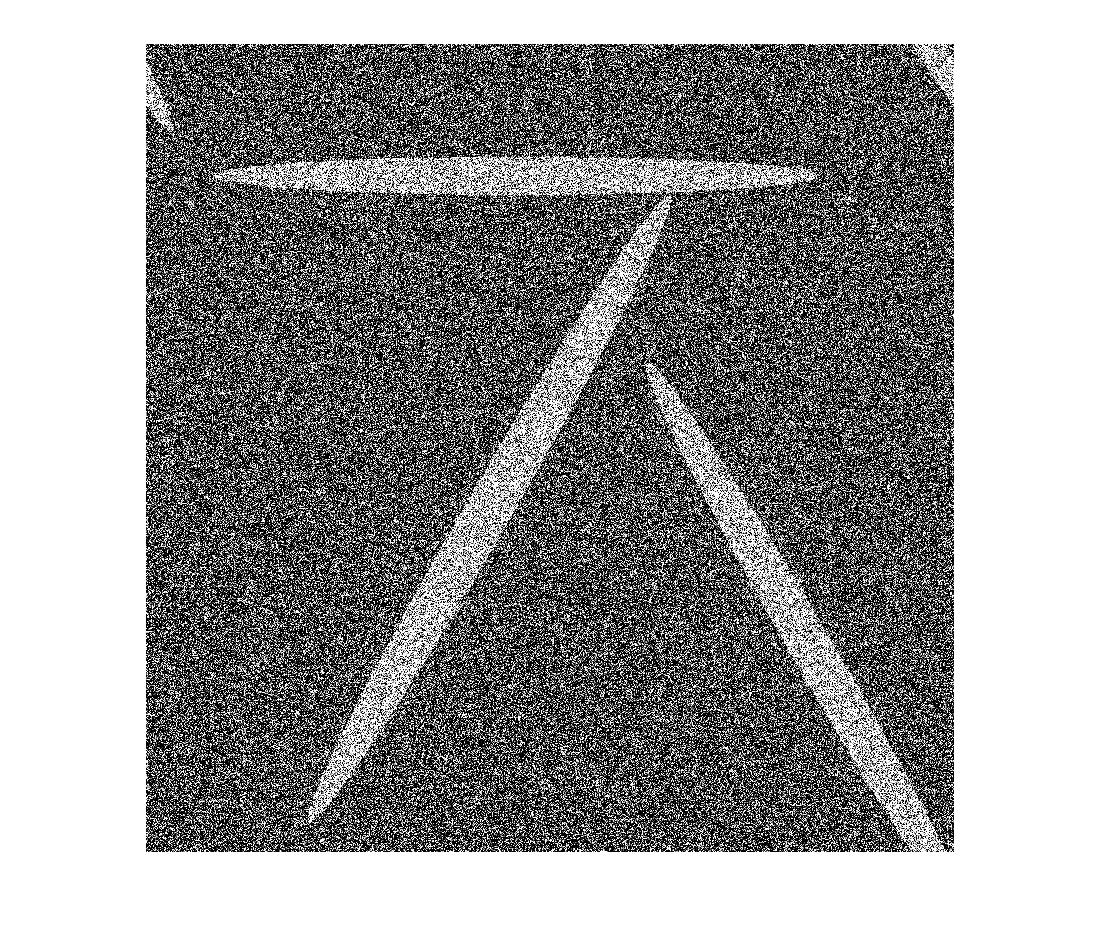
\includegraphics[scale=.17]{../../figs/ellipses_t1}
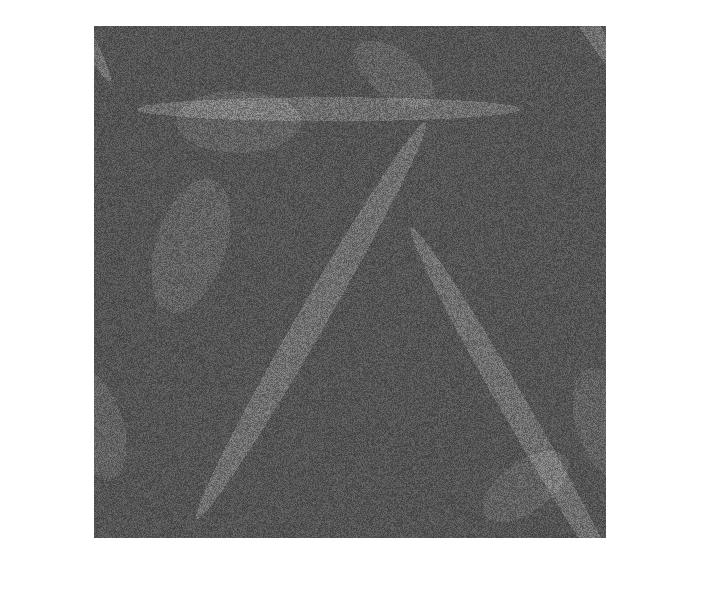
\includegraphics[scale=.17]{../../figs/ellipses_t2}
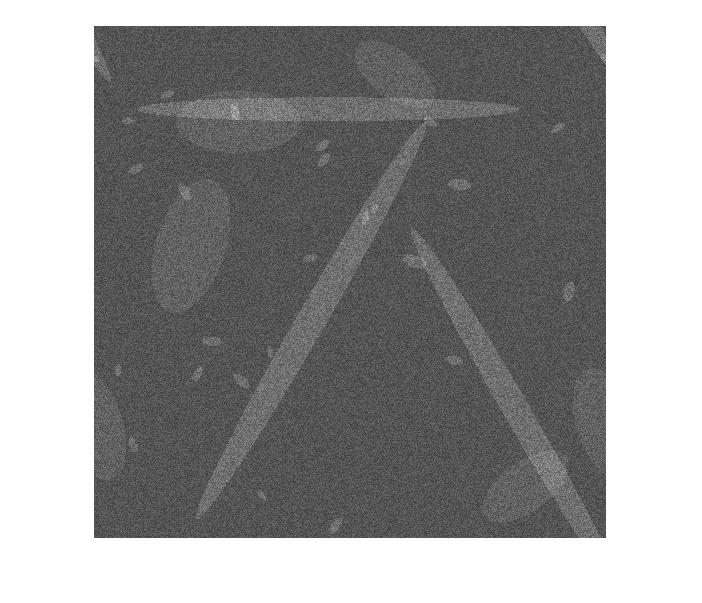
\includegraphics[scale=.17]{../../figs/ellipses_t3}
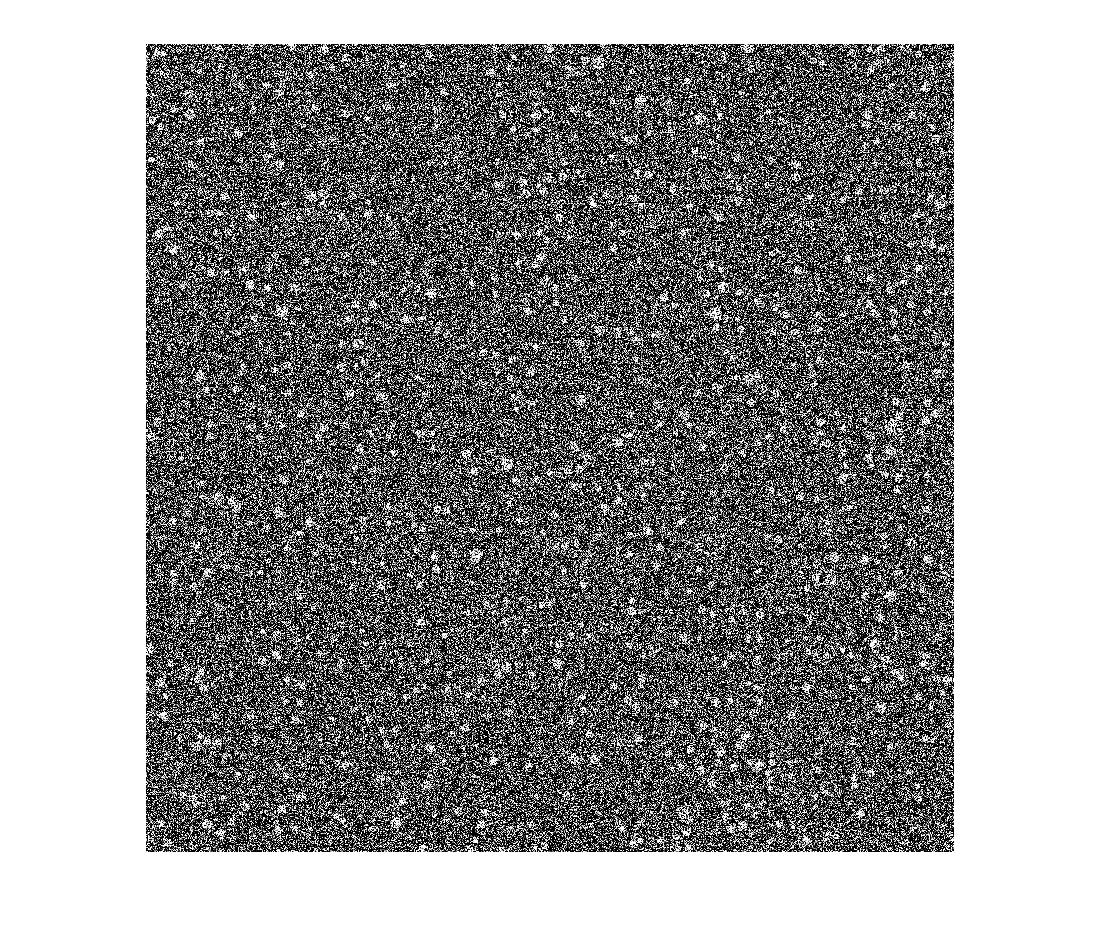
\includegraphics[scale=.17]{../../figs/ellipses_t4}
\caption{Synthetic multi-temporal ($n=4$) images. Features and changes come as ellipses and dots.}
\label{F:EllipsoidChanges}
\end{figure}


\begin{figure}[htp!]
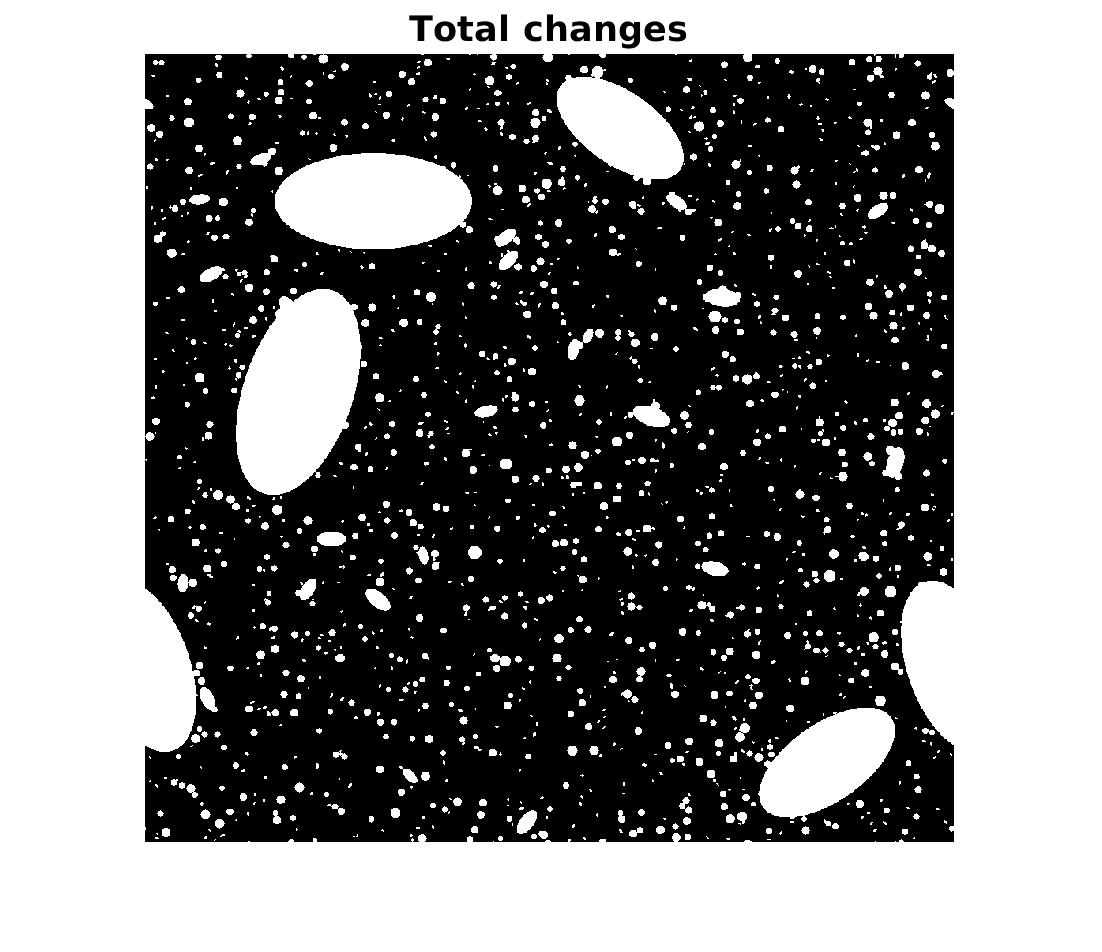
\includegraphics[scale=.1]{../../figs/total_changes}(a)
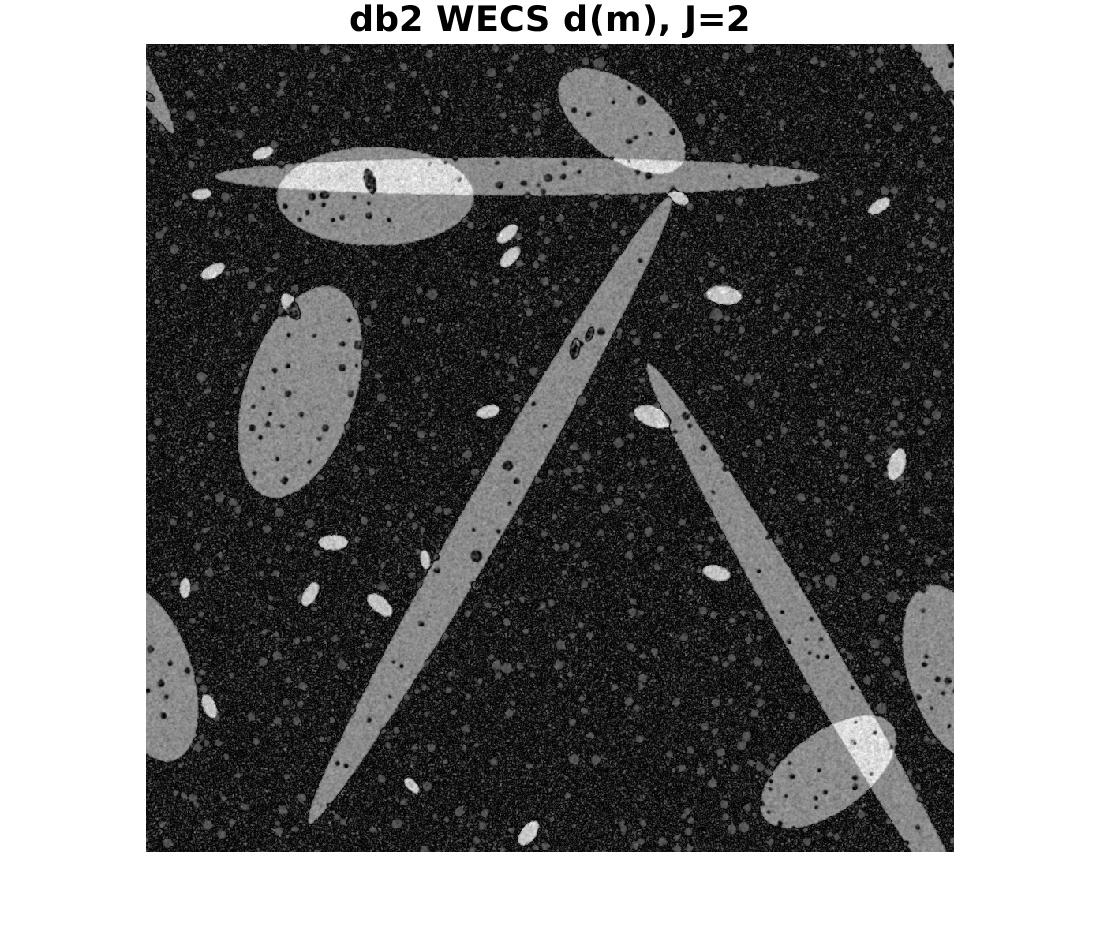
\includegraphics[scale=.1]{../../figs/corr_changes_dm}(b)
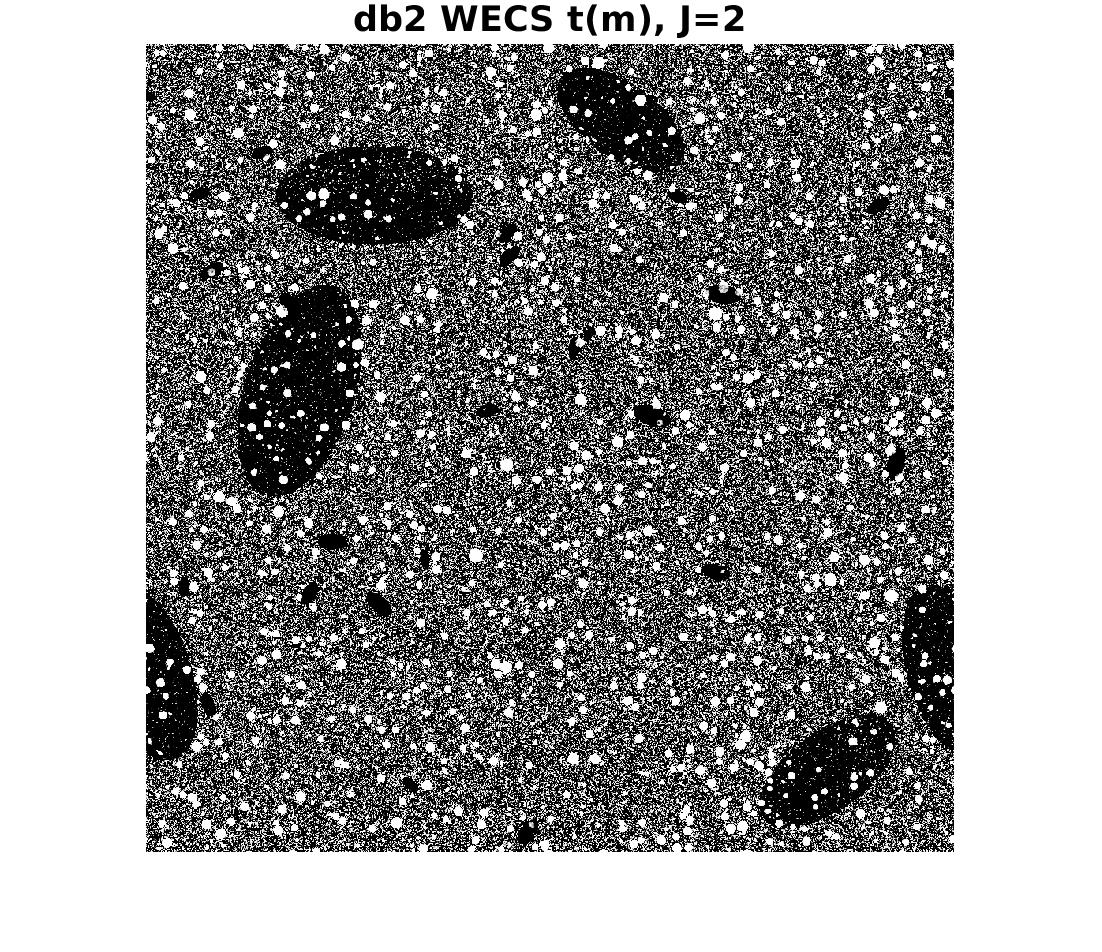
\includegraphics[scale=.1]{../../figs/corr_changes_tm}(c)
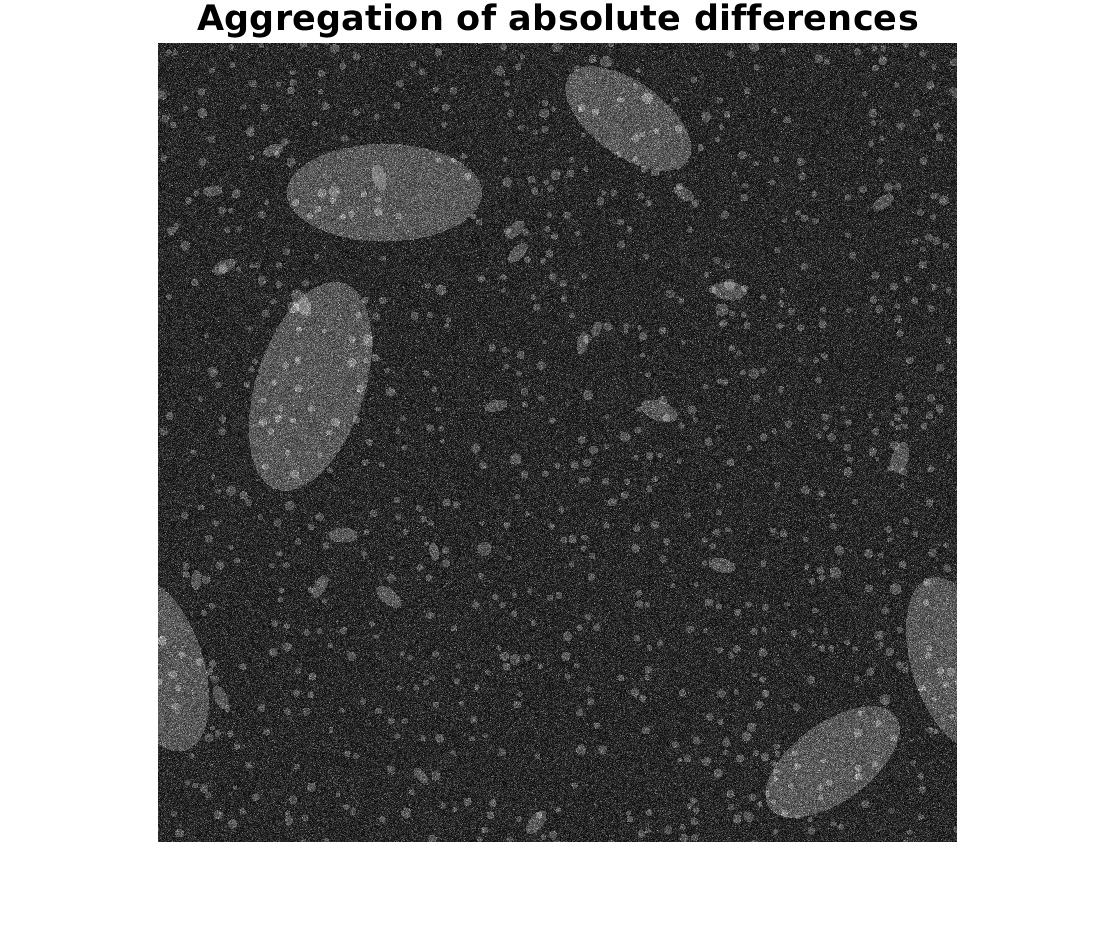
\includegraphics[scale=.1]{../../figs/corr_changes_logratios}(d)
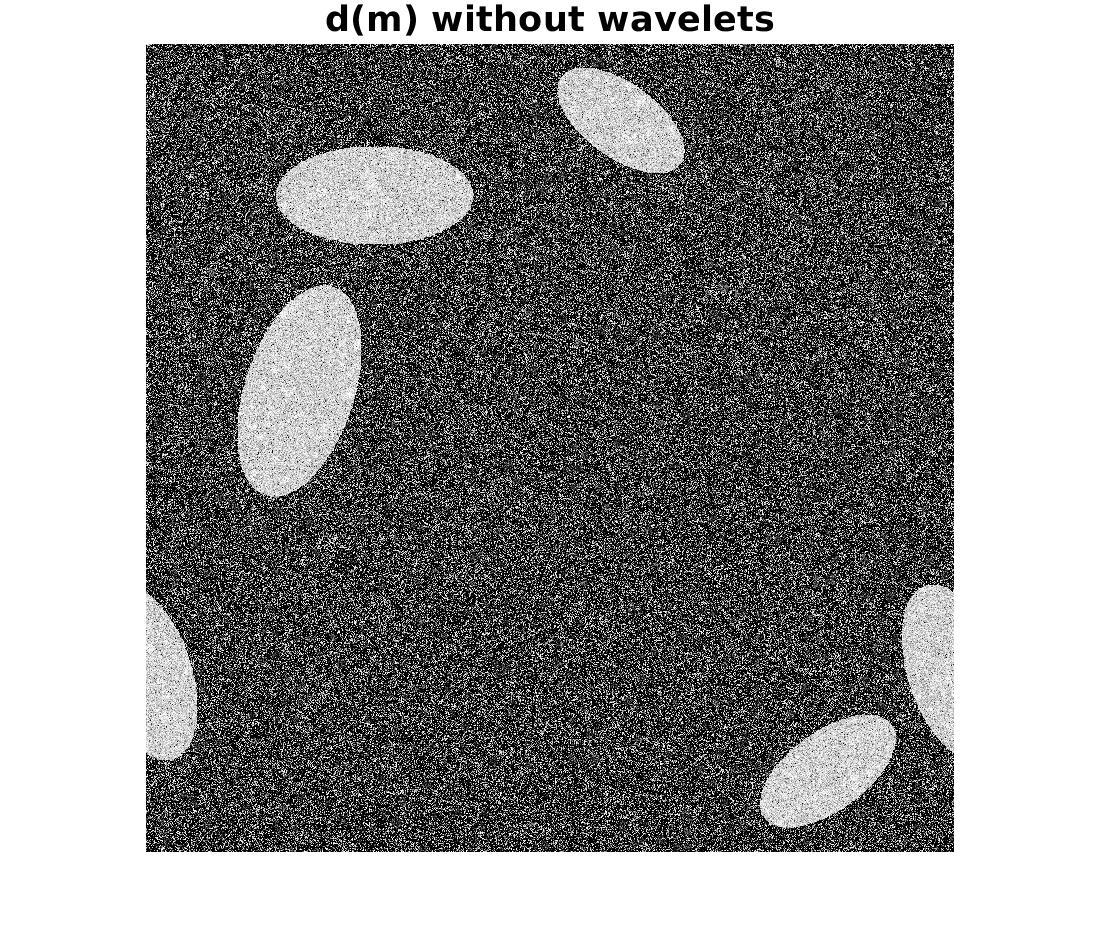
\includegraphics[scale=.1]{../../figs/corr_changes_dm_nowavelets}(e)
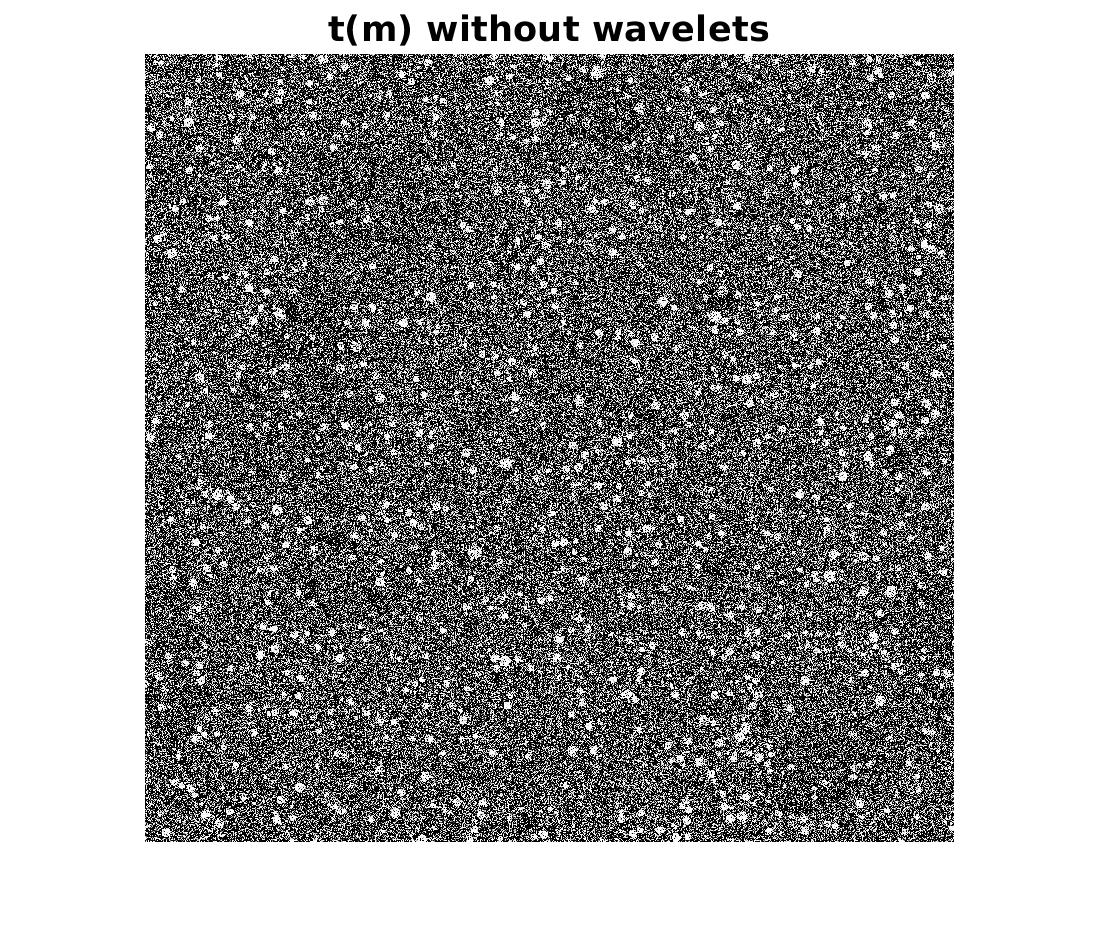
\includegraphics[scale=.1]{../../figs/corr_changes_tm_nowavelets}(f)
\caption{Synthetic images with changing ellipses. (a) Image composed by the total changes over time. 
(b) Proposed db2 WECS $\vd(m)$ with $J=2$; (c) Proposed db2 WECS $\vt(m)$ with $J=2$.
(d) Standard approach. (e) $\vd(m)$ without wavelets. (f) $\vt(m)$  without wavelets. 
}
\label{F:Changes_methods_images}
\end{figure}

Figure \ref{F:Changes_methods_images} illustrates the simulated synthetic images, the proposed wavelet detection methods, and three classic detection methods, as well. Panel (a) presents the total changes with respect to image $I(1)$. Panels (b) and (c) show the results by the proposed methods using Daubechies wavelet with two null moments (db2) and $J=2$ by $\vd(m)$ and $\vt(m)$, respectively. Panel (d) presents the results by a standard approach (aggregated log-ratios). Finally, in Panels (e) and (f)  we can see the results if $\vd(m)$ and $\vt(m)$ are performed purely on the spatial domain, without multiscale approximations. The spatio-temporal advantages of the proposed wavelet  $\vd(m)$ and $\vt(m)$ are clear in Figure \ref{F:Changes_methods_images}. A slight advantage for the detection of small ellipses is attained by $\vd(m)$ over $\vt(m)$.   


We compute ROC curves to compare the detection performance of different methods. For this we simulate noisy versions of the synthetic images illustrated by Figure \ref{F:EllipsoidChanges}. The change detection methods are then employed. Each method generates a correlation matrix between the real image of total changes and the estimated one.

Each ROC curve presents how close the magnitude variation of change measures is to the variation of the image of total changes in the following way:
\begin{enumerate}
\item Let $R$ be the matrix of change measures. Compute the range $[r_{\min},r_{\max}]$ of the values in $R$;
\item Let $(r_{(1)},\ldots,r_{(100)})$ be equally space values between $r_{\min}$ and $r_{\max}$;
\item For each $k=1,\ldots,n$, check how many pixels are such that $R_{i,j}>r_{(k)}$ coincide with the pixels $(i,j)$ where a change really occurs on the image of total changes. Dividing this number by the total number of changes gives the true positive rate.
\item For each $k=1,\ldots,n$, check how many pixels are such that $R_{i,j}>r_{(k)}$  do not coincide with the pixels $(i,j)$ where a change really occurs. Dividing this number by the total number of pixels where changes do not occur gives the false positive rate.
\end{enumerate}

\begin{figure}[htp!]
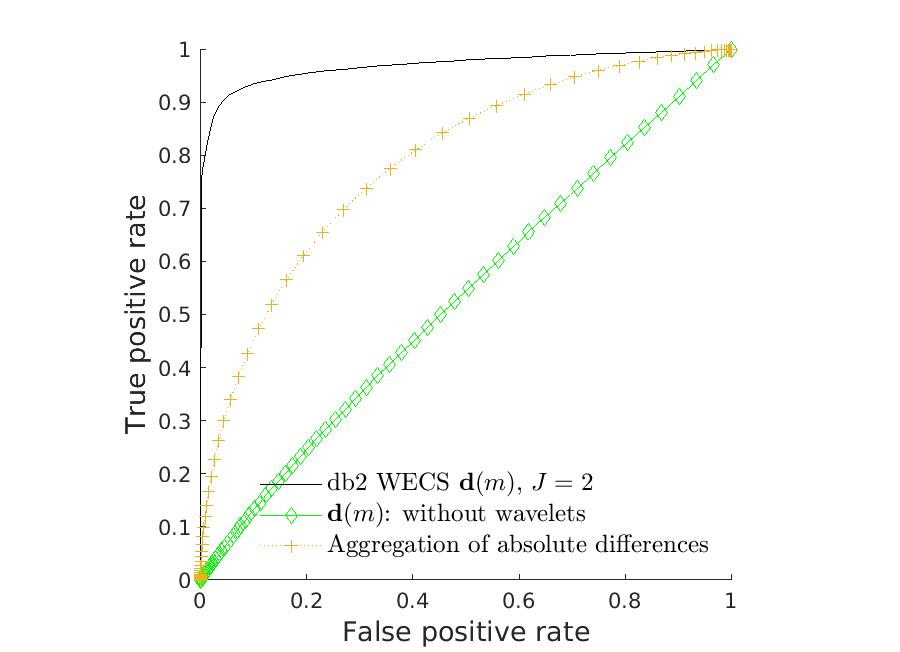
\includegraphics[scale=.13]{../../figs/methods_comparison}\hspace{-.5cm}(a) 
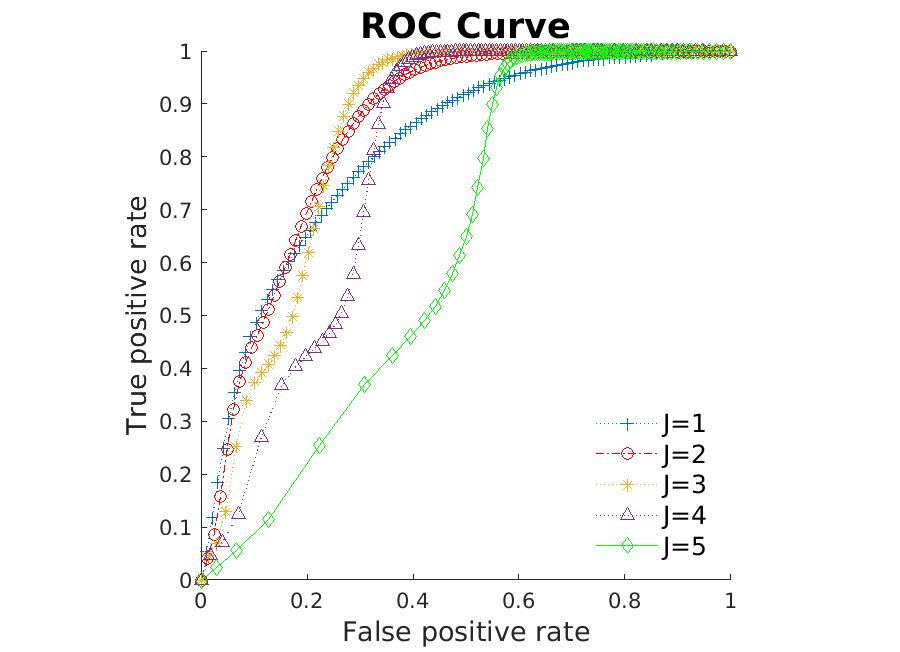
\includegraphics[scale=.13]{../../figs/levels_comparison_WithReference}\hspace{-.5cm}(b)\\
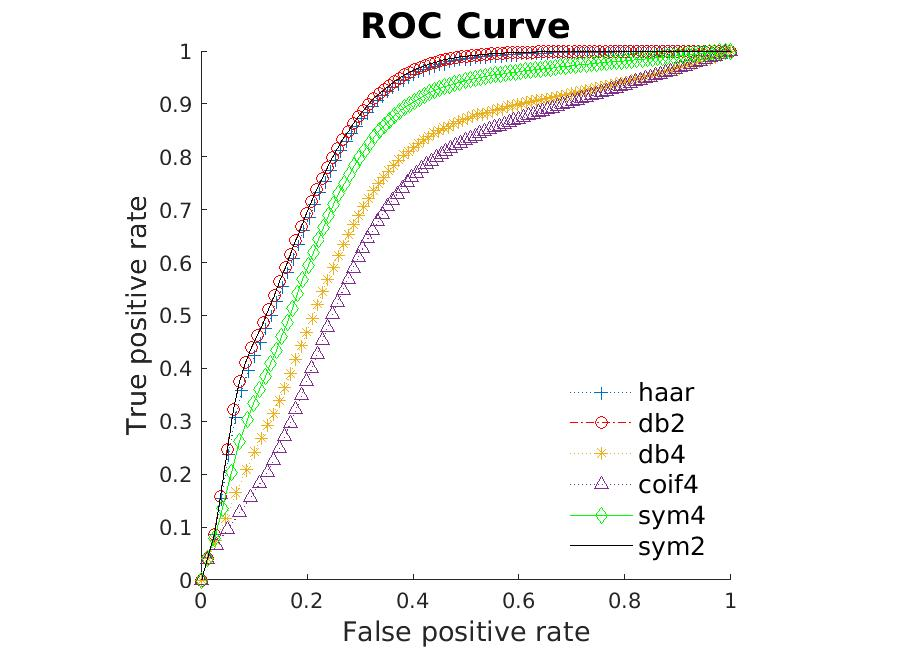
\includegraphics[scale=.13]{../../figs/families_comparison_WithReference}\hspace{-.5cm}(c)
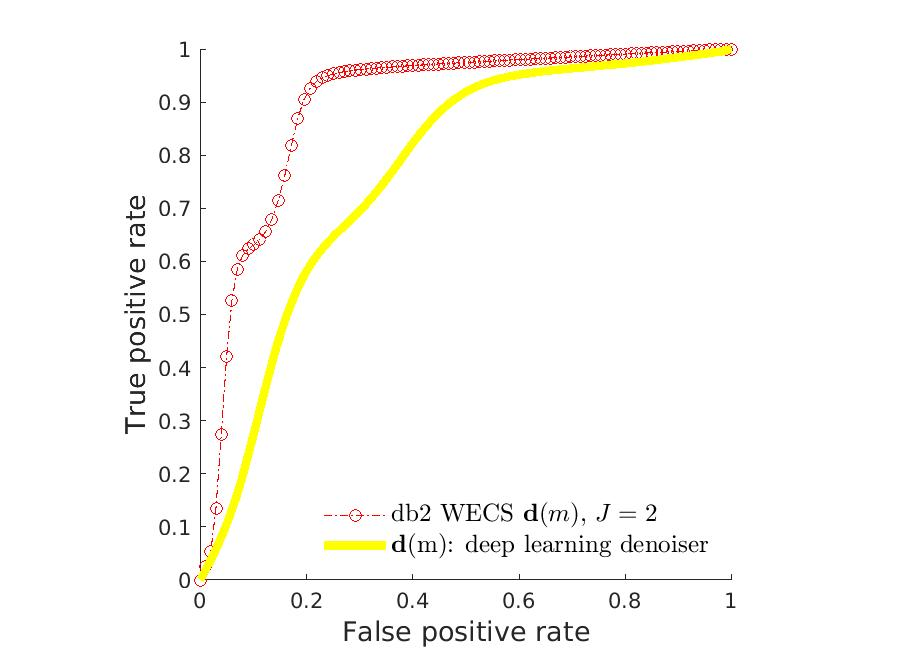
\includegraphics[scale=.13]{../../figs/dm_comparison_wavelet_deepL}\hspace{-.5cm}(d) \\
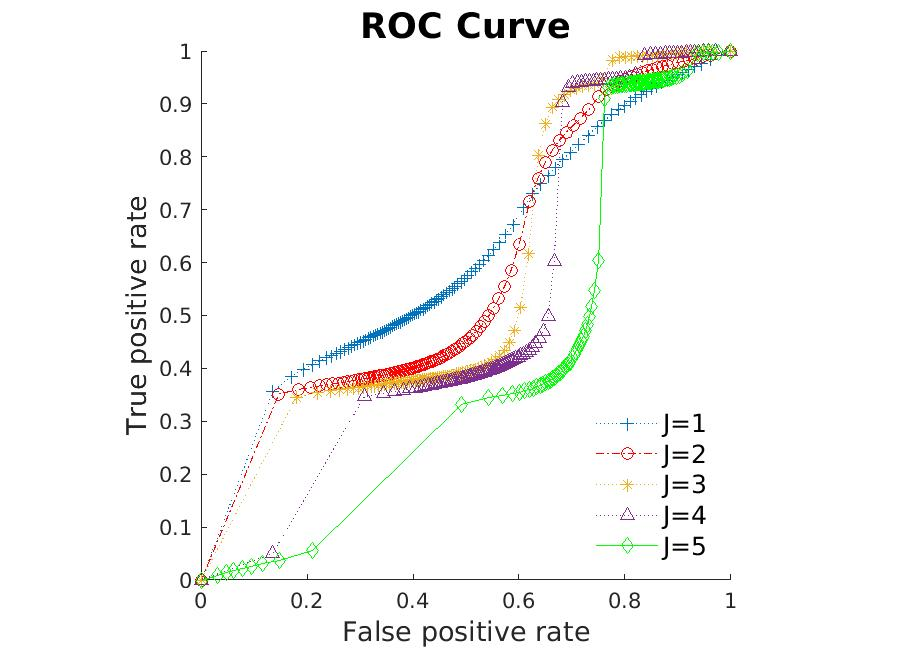
\includegraphics[scale=.13]{../../figs/levels_comparison_NoReference}\hspace{-.5cm}(e)
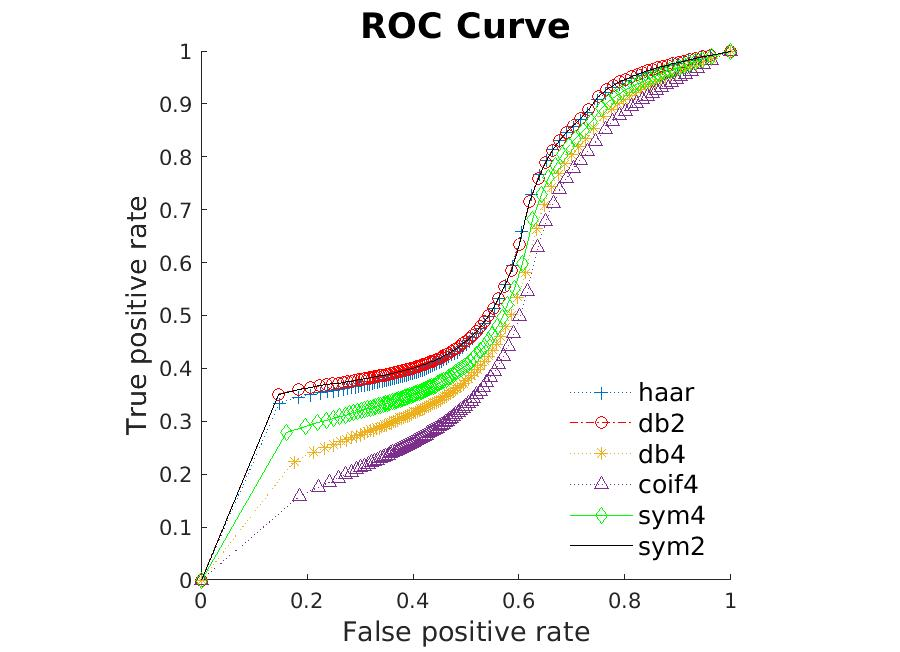
\includegraphics[scale=.13]{../../figs/families_comparison_NoReference}\hspace{-.5cm}(f)
\caption{ROC curves for detection of changing ellipses in synthetic images and different methods. (a) The proposed methods in black (db2 WECS $\vd(m)$) and green (db2 WECS $\vt(m)$) vs three non-wavelet methods: standard (red stars); $\vd(m)$ (blue); and $\vt(m)$ (red circles). 
(b) db2 $\vd(m)$ with different levels.
(c) $\vd(m)$ with different wavelet bases and J=2;
(d) The proposed db2 WECS $\vd(m)$ (red circles) and $\vd(m)$ with deep-learning feature extraction and without wavelets (yellow line).  
(e) db2 $\vt(m)$ with different levels. (f) $\vt(m)$ with different wavelet bases and J=2. }
\label{F:EllipsoidChanges_details}
\end{figure}

Figure \ref{F:EllipsoidChanges_details} presents the different ROC curves for change detection methods applied to the synthetic data as follows. The effects of wavelet bases, level of decomposition, deep-learning feature extraction and $\vd(m)$/$\vt(m)$ usage are shown on the ROC curves. We employ the following wavelet bases: Haar;  Daubechies db2; Daubechies db4; Coiflets coif4; Symlets sym2 ; and Symlets sym4. Panels (c) and (f) present the ROC curves for the proposed methods under the aforementioned bases for $\vd(m)$ and $\vt(m)$, respectively. On both instances $J=2$ is employed. The results for $\vd(m)$ are much more robust to basis variation than the ones for $\vt(m)$. Combining the ROC curves's comparison from both panels, Daubechies db2 is the best choice.  Panels (b) and (e) present the ROC curves for different levels of decomposition under the aforementioned bases for $\vd(m)$ and $\vt(m)$, respectively. On both instances db2 is employed, and five levels are considered: $J=1,2,3,4,5$. Levels $J=2,3$ have a clear better performance for $\vd(m)$ (with a slight advantage to $J=2$), whilst $J=1$ is competitive for $\vt(m)$. The overall performance  of $J=2$ warrants its use for the rest of the comparisons. Panel (d) shows how the proposed method performs with or without images' deep learning feature extraction from a residual learning network \cite{zhang2017beyond}. The change detection method is the proposed db2 $\vd(m)$ with $J=2$. We can see that the ROC curves for images treated with deep-learning methods or treated with wavelet based methods are almost identical. The WECS runs in 3.35s, while the deep-learning based $\vd(m)$ runs in 559.12s on a notebook. The configuration of the notebook is: OS - Ubuntu 18.04.5 LTS; RAM 7.7 GB; Intel\textregistered Core\texttrademark $ $i7-7500U CPU @ 2.70GHz x 4; graphics - Intel\textregistered HD Graphics 620 (KBL GT2); GNOME - 3.28.2; OS type - 64-bit. We finally have in Panel (a) the proposed db2 $\vd(m)$ with $J=2$ and db2 $\vt(m)$ with $J=2$  compared to three other non-wavelet methods. These are $\vd(m)$ and $\vt(m)$ where wavelet decomposition is not performed, i.e., the squared deviations are computed using $\{\mathcal{I}(m)\}$ instead of $\{\vX(m)\}$, and the classic method of analyzing aggregated log-ratios of $\{\mathcal{I}(m)\}$. The ROC curves in Panel (a) clearly show that  the proposed db2 $\vd(m)$ with $J=2$ outperforms the rest. 

We may summarize these results as: the proposed wavelet $\vd(m)$ method presents a superior performance. It is also equipped with the following nice properties: (i) it is scalable; (ii) it is sparse; (iii) it is parsimonious; (iv) it can be easily adapted to be linearly updated when a new image is acquired; and (v) it is fast. Hence, the proposed wavelet change-detection procedure can be used as a real-time change detection tool for long time series of large images.    




\section{Real Data Results}\label{section_realdata}

We employed the proposed change detection method on a series of 85 multi-date satellite images. The images were taken on a forest region at the border of Brazil and the French Guiana from November 08, 2015 to December 09, 2017. Each image has two channels and 1200 by 1000 pixels. We perform three change detection wavelet analyses: VV Polarization Channel;  VH Polarization Channel; and the Combined Image by Euclidean norm. 

A multi-resolution analysis (MRA) based on a Symlet basis with filter of length 16 (symlet 8) is built.  The log-images are approximated at levels $J=1,2,3,4$. Table \ref{T:approxenergy} shows the 85 images' average energy for each approximation level. We notice that roughly 99\% of the energy is recovered with $J=1$, and more than  90\% with $J=2$. The VV channel shows better overall energy recovery than the VH channel. For $J=4$ and $J=3$, the Euclidean combination of the polarization channels increases the energy representation percentage.  For $J=2$, VV channel and combined channels are equivalent. VH has 4\% less energy than VV for $J=3$, and $10\%$ less  for $J=4$.

\begin{table*}[h!]
\caption{Wavelet Approximation Mean Energy Percentage for log-images. Forest region at the border of Brazil and the French Guiana from November 08, 2015 to December 09, 2017. $n=85$ multi-date satellite images. Each image has two channels and 1200 by 1000 pixels. VV Polarization Channel;  VH Polarization Channel; and the Combined Image by Euclidean norm. Approximation $J=1,2,3,4$.}
\centering
\begin{tabular}{cccc|cccc|cccc}
\hline
\multicolumn{12}{c}{\sc Mean Approximated Energy Percentage}\\
\hline
\multicolumn{4}{c|}{VV Channel}&\multicolumn{4}{c|}{VH Channel}&\multicolumn{4}{c}{Combined Channels}\\
\hline
$J=4$&$J=3$&$J=2$&$J=1$&$J=4$&$J=3$&$J=2$&$J=1$&$J=4$&$J=3$&$J=2$&$J=1$\\
\hline
0.803&0.847&0.924&0.990&0.763&0.814&0.908&0.988&0.816&0.858&0.931&0.991\\
\hline
\end{tabular}\label{T:approxenergy}
\end{table*}

Figures \ref{F:squared_J1-4_VV}-\ref{F:squared_J1-4_euclid} show the series of squared deviations $\vd(m)$ and $\vt(m)$, for  the VV channel, VH channel, and Euclidean combination, respectively.  An overall feature on this data is that the VV polarization presents much higher energy than the VH. The amount of energy related to changes  is ten times higher on the former compared to the latter's.

Regarding change time points, in each figure, we can notice a pattern of peaks which are common to all approximation levels. They are time points:
\begin{list}{}{}
\item (a) 14, 43, 54, and 58 by the coefficients' squared deviations on the average VV image;
\item (b) 14, 43, 54, and 58 by the coefficients' squared deviations on the consecutive VV images;
\item (c) 14, 38, 41, 43, 54, 56, and 58 by the coefficients' squared deviations on the average VH image;
\item (d) 14, 38, 41, 43, 54-58 by the coefficients' squared deviations on the consecutive VH images;
\item (e) 14, 43, 54, and 58 by the coefficients' squared deviations on the average combined channels image; and
\item (e) 14, 43, 54, and 58 by the coefficients' squared deviations on the consecutive combined channels images.
%%%%%%%% VV 12 14 15 16 (42) 43 54 56 58 d(m)
%%%%%%%% VV 12 14 15 16 (42) 43 54 56 58 t(m)
%%%%%%%% VH  12 14 15 38 41 43 54 56 58
%%%%%%%% euclid 12 14 15 16 43 54 56 58
\end{list}

\begin{figure}[htp!]
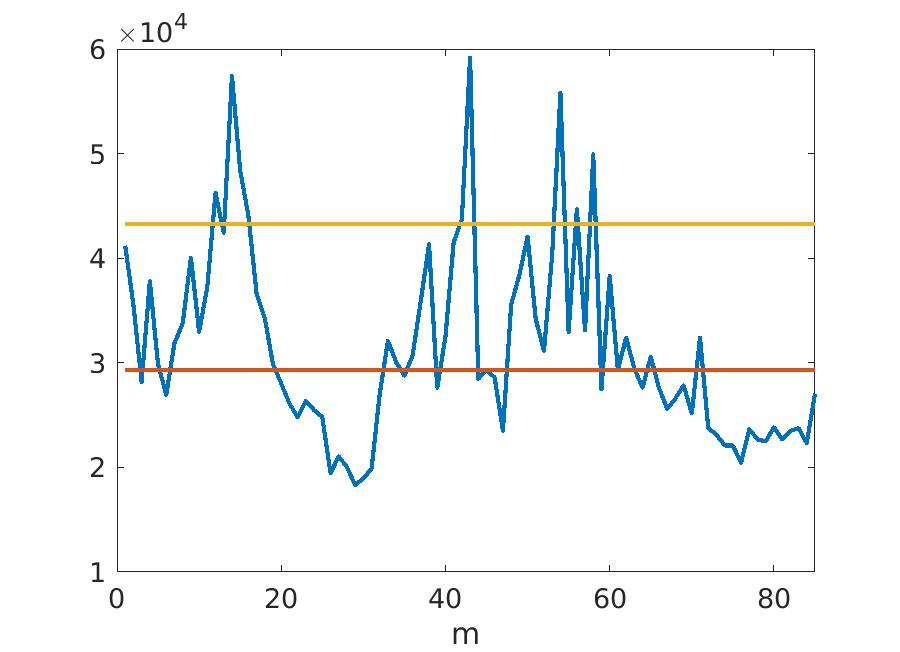
\includegraphics[scale=.12]{../../figs/J1_VV_squared_meandev}(a)
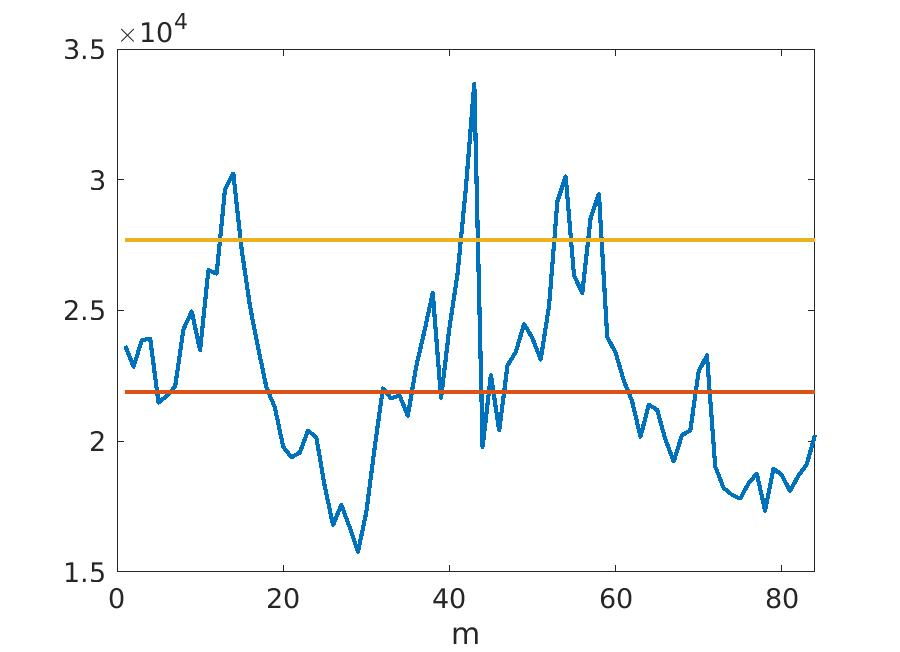
\includegraphics[scale=.12]{../../figs/consecdif_J1_VV_squared_meandev}(b)\\
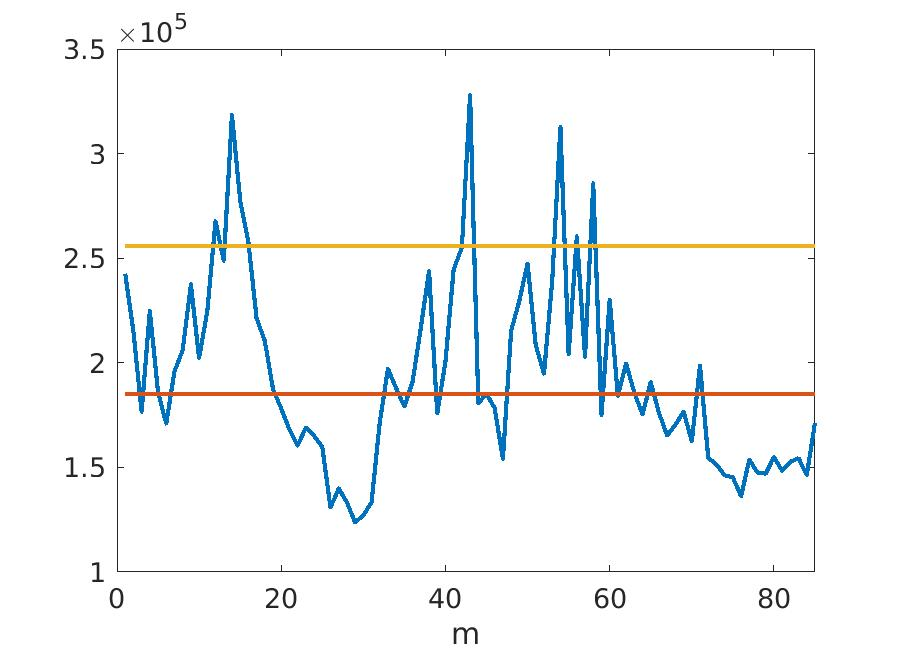
\includegraphics[scale=.12]{../../figs/J2_VV_squared_meandev}(c)
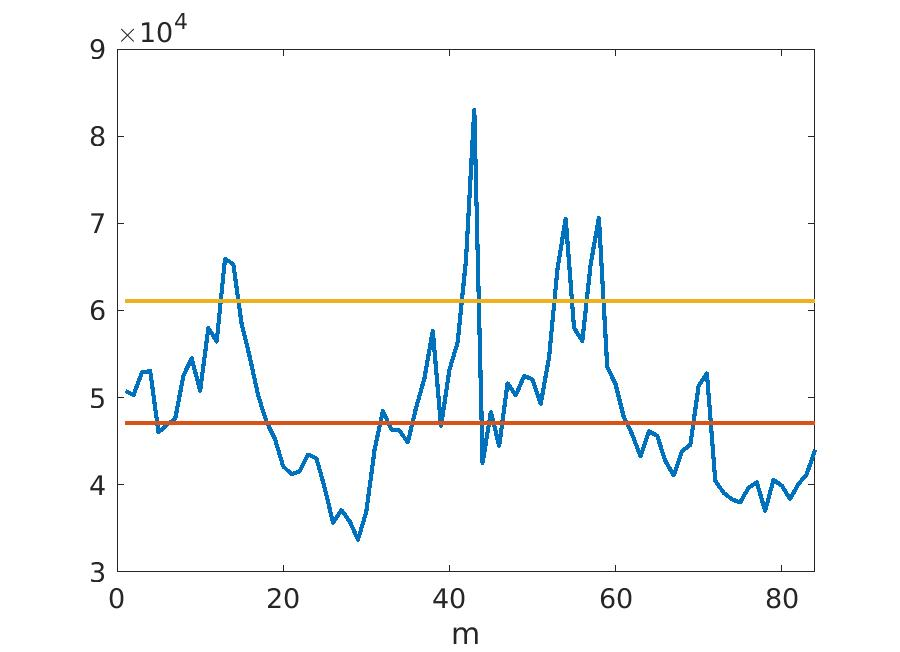
\includegraphics[scale=.12]{../../figs/consecdif_J2_VV_squared_meandev}(d)\\
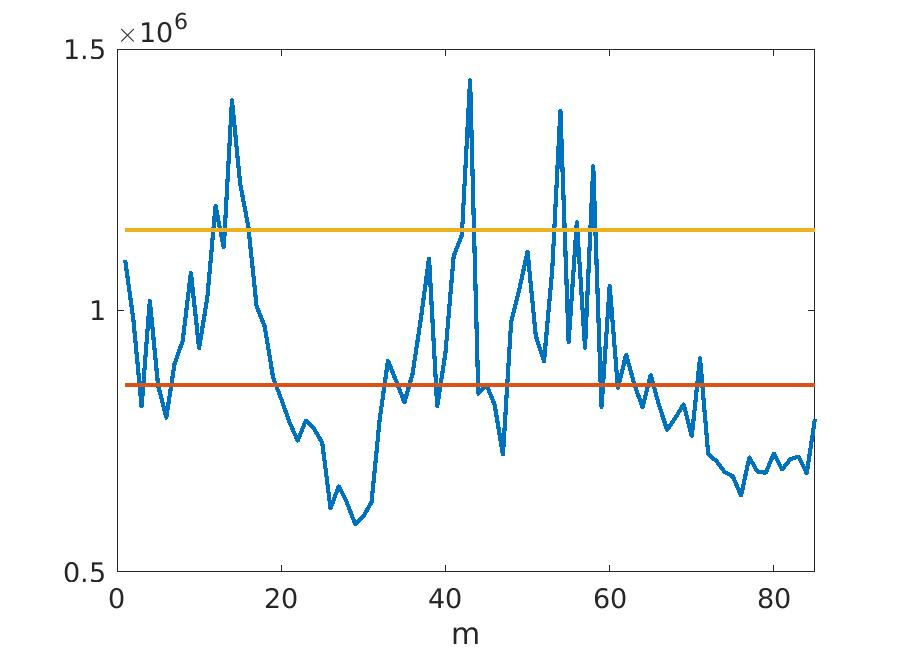
\includegraphics[scale=.12]{../../figs/J3_VV_squared_meandev}(e)
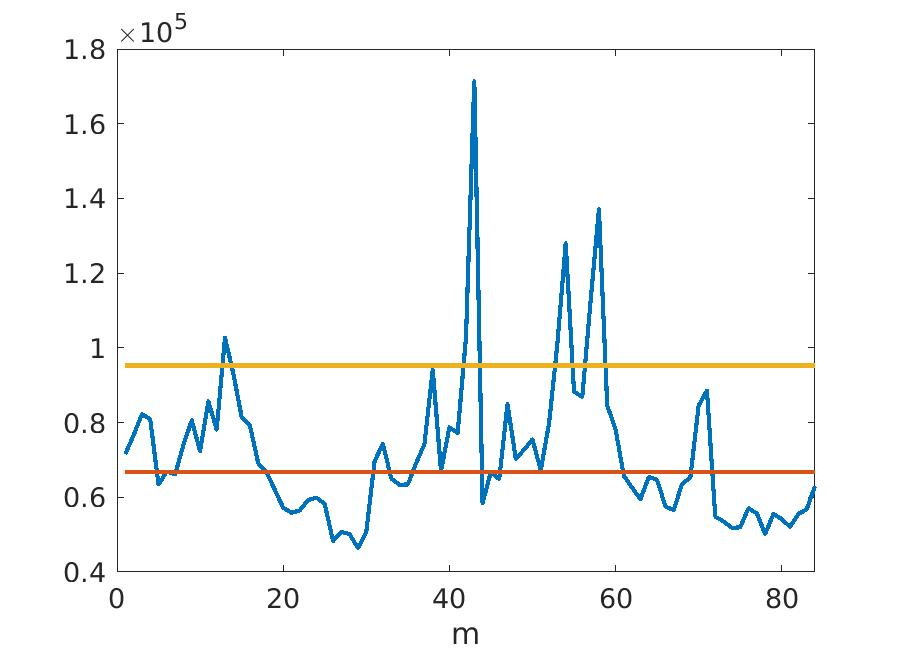
\includegraphics[scale=.12]{../../figs/consecdif_J3_VV_squared_meandev}(f)\\
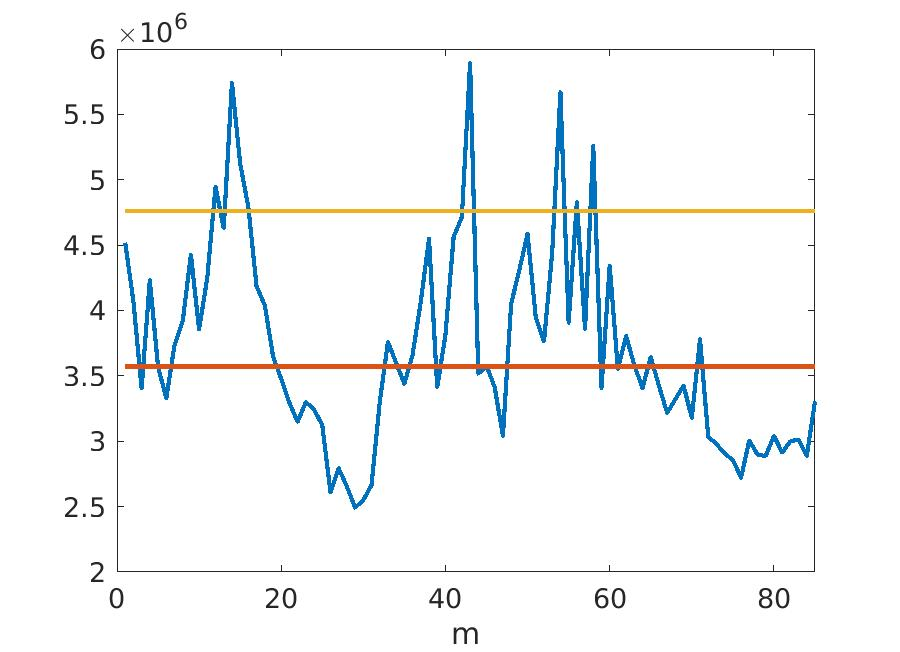
\includegraphics[scale=.12]{../../figs/J4_VV_squared_meandev}(g)
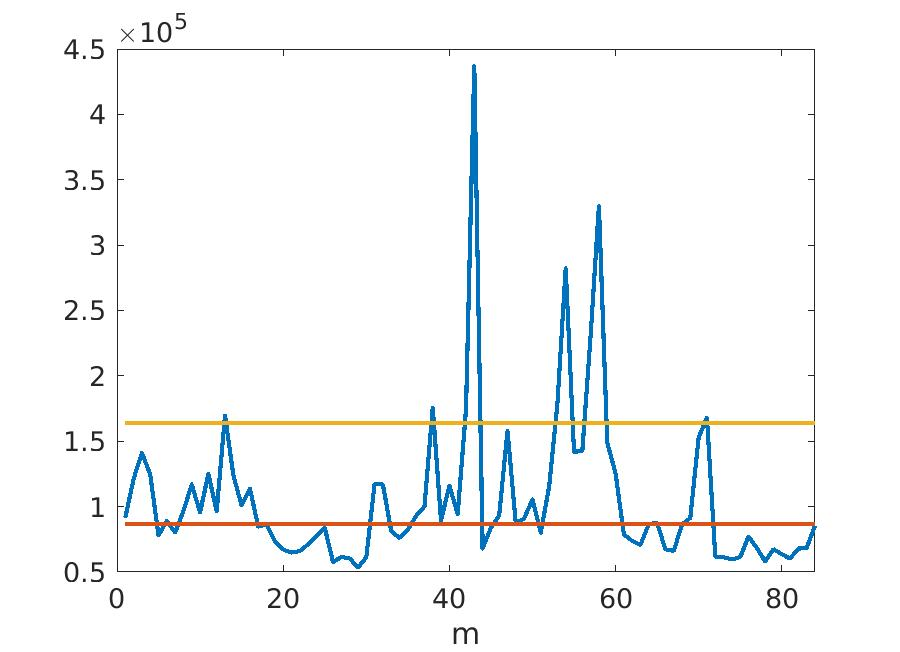
\includegraphics[scale=.12]{../../figs/consecdif_J4_VV_squared_meandev}(h)
\caption{{\sc VV Polarization Channel} Series of squared deviations $\vd(m)$ and $\vt(m)$. The red horizontal line represents the median value and the yellow horizontal line represents their median plus two times their absolute median deviation.  $\vd(m)$ - Approximation Levels:  (a) $J=1$; (c) $J=2$; (e) $J=3$; (g) $J=4$. $\vt(m)$ - Approximation Levels:  (b) $J=1$; (d) $J=2$; (f) $J=3$; (h) $J=4$. 
}
\label{F:squared_J1-4_VV}
\end{figure}

\begin{figure}[htp!]
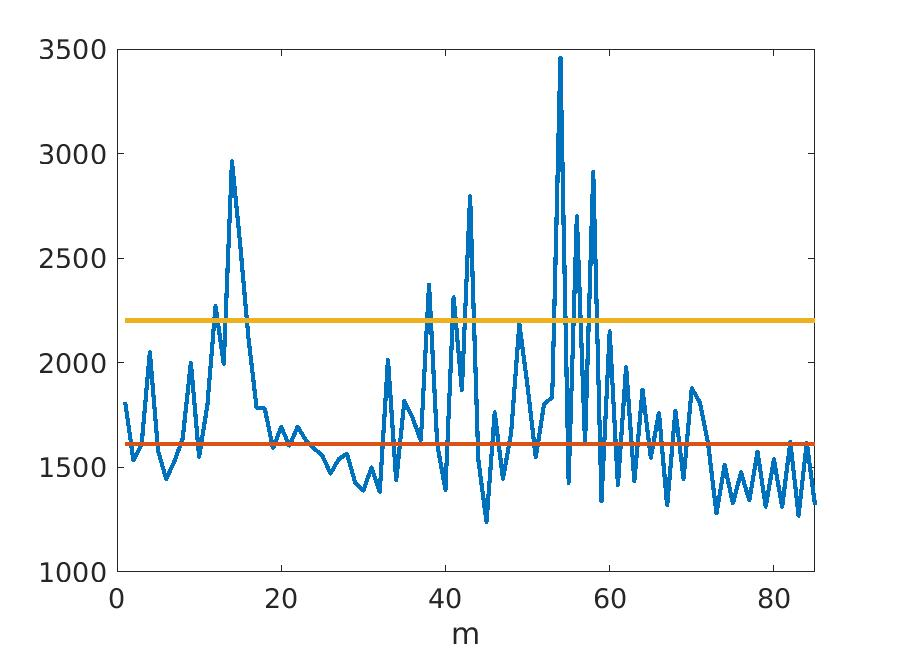
\includegraphics[scale=.12]{../../figs/J1_VH_squared_meandev}(a)
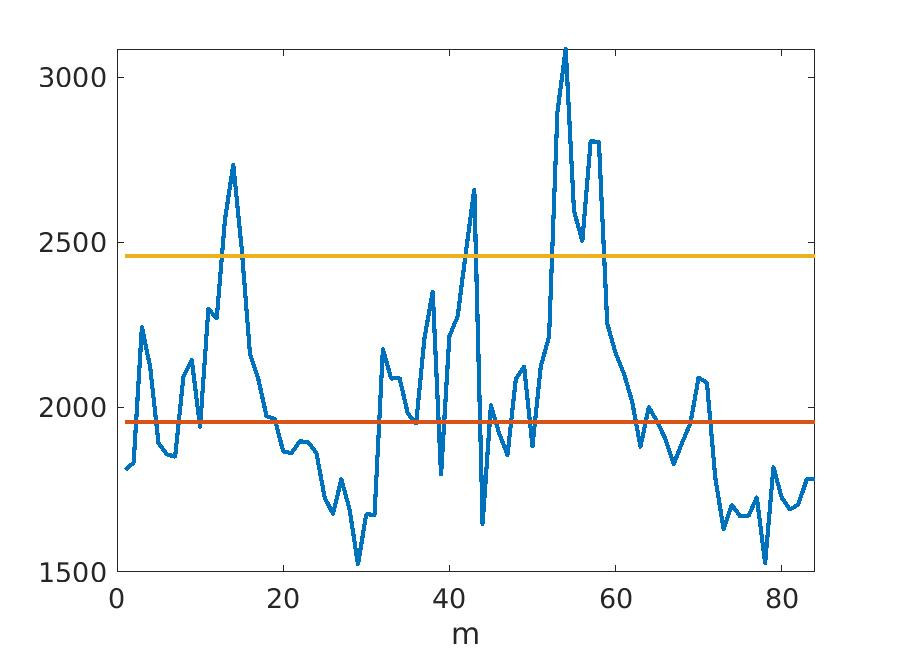
\includegraphics[scale=.12]{../../figs/consecdif_J1_VH_squared_meandev}(b)\\
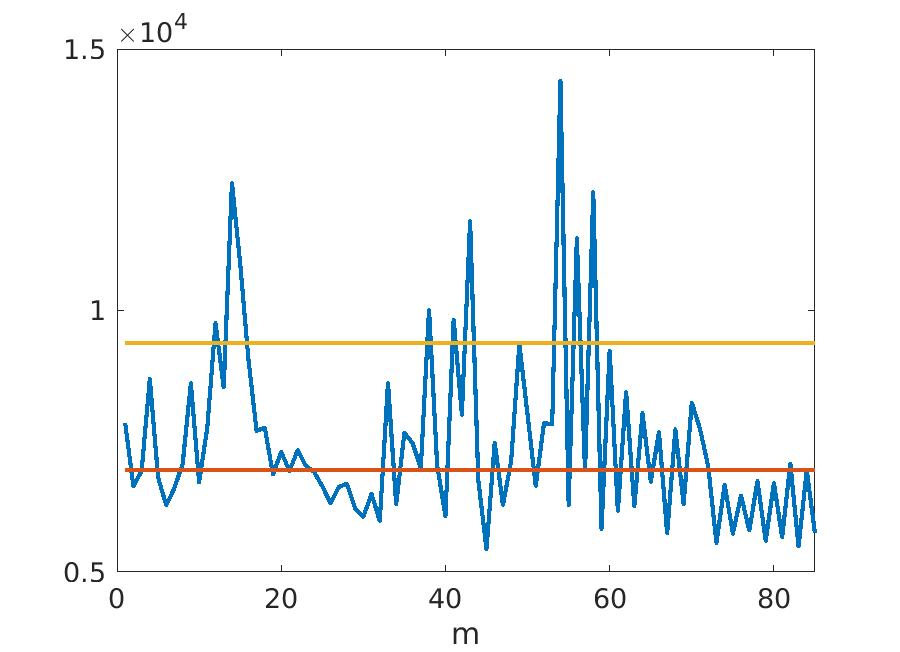
\includegraphics[scale=.12]{../../figs/J2_VH_squared_meandev}(c)
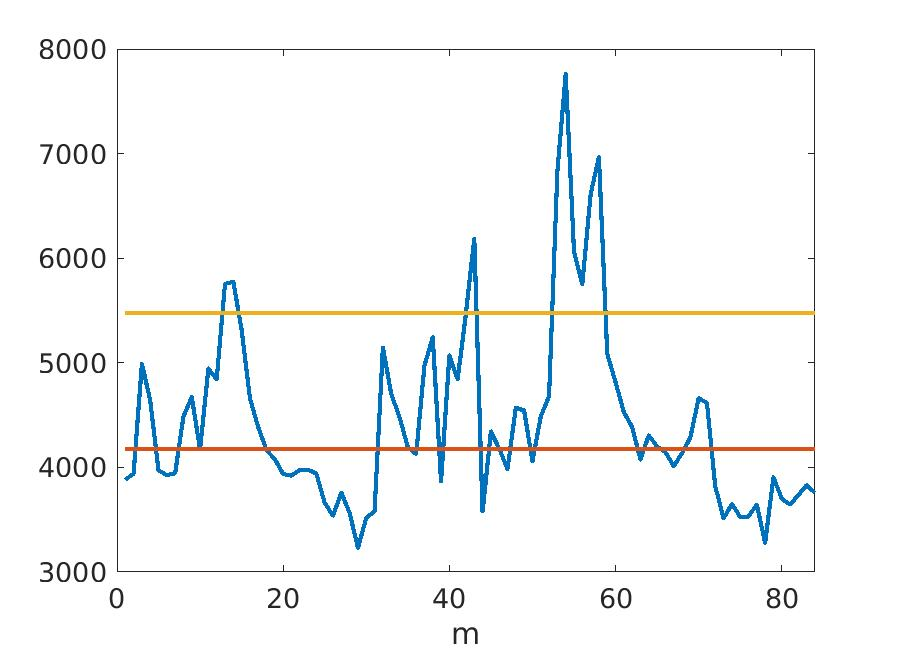
\includegraphics[scale=.12]{../../figs/consecdif_J2_VH_squared_meandev}(d)\\
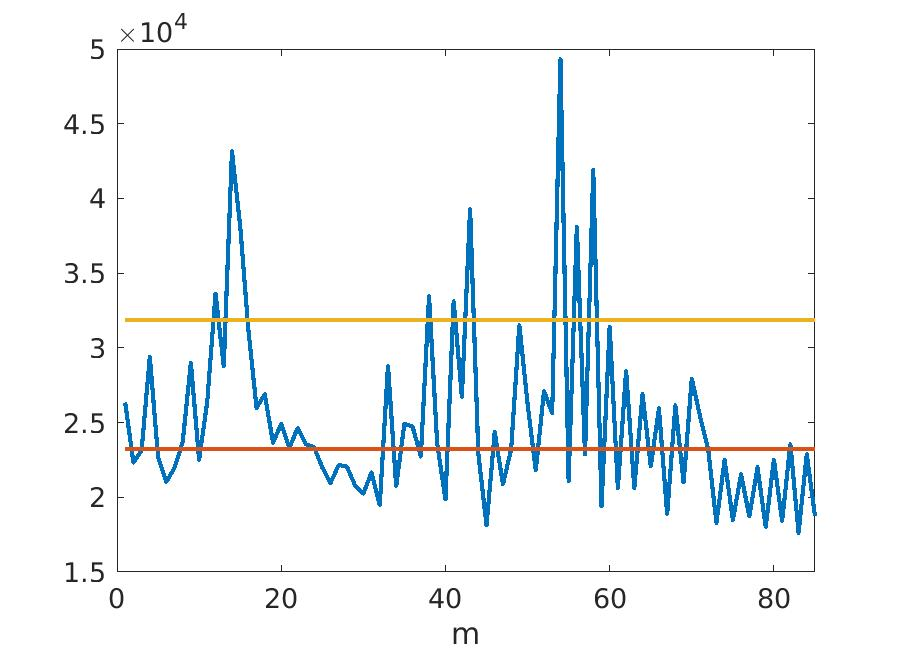
\includegraphics[scale=.12]{../../figs/J3_VH_squared_meandev}(e)
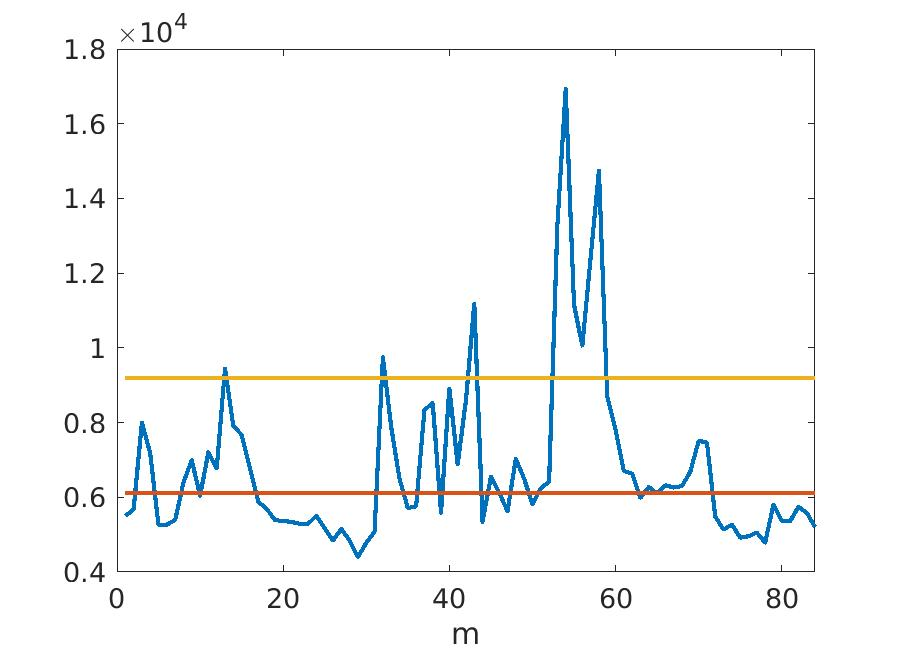
\includegraphics[scale=.12]{../../figs/consecdif_J3_VH_squared_meandev}(f)\\
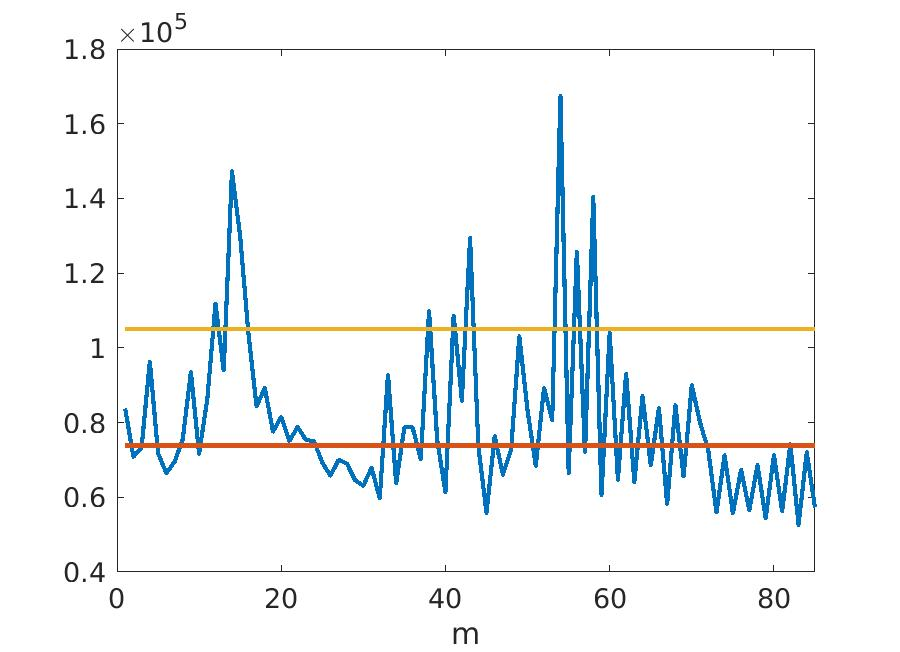
\includegraphics[scale=.12]{../../figs/J4_VH_squared_meandev}(g)
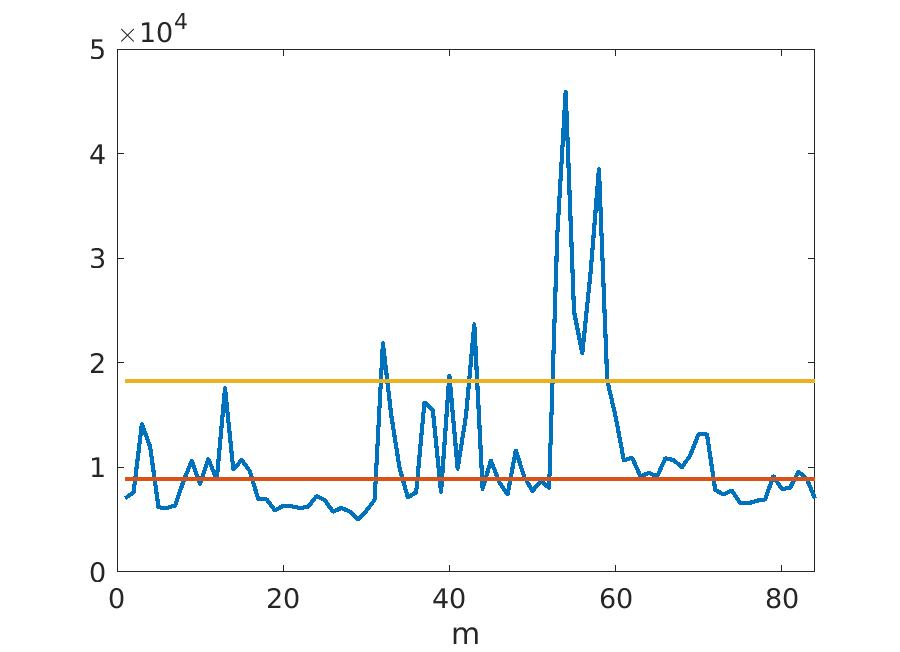
\includegraphics[scale=.12]{../../figs/consecdif_J4_VH_squared_meandev}(h)
\caption{{\sc VH Polarization  Channel} Series of squared deviations $\vd(m)$ and $\vt(m)$. The red horizontal line represents the median value and the yellow horizontal line represents their median plus two times their absolute median deviation.  $\vd(m)$ - Approximation Levels:  (a) $J=1$; (c) $J=2$; (e) $J=3$; (g) $J=4$. $\vt(m)$ - Approximation Levels:  (b) $J=1$; (d) $J=2$; (f) $J=3$; (h) $J=4$. 
}
\label{F:squared_J1-4_VH}
\end{figure}

\begin{figure}[htp!]
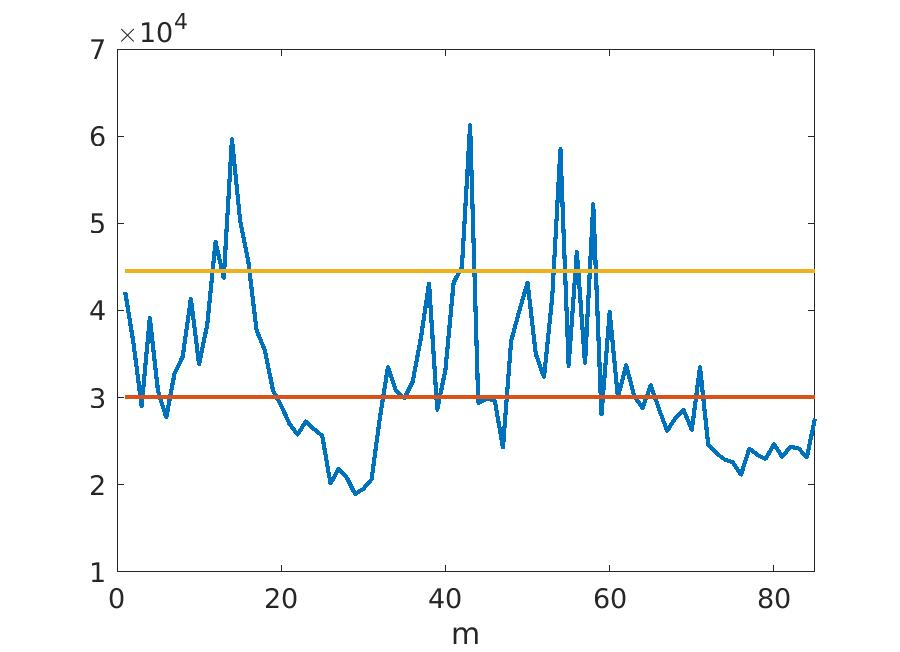
\includegraphics[scale=.12]{../../figs/J1_euclid_squared_meandev}(a)
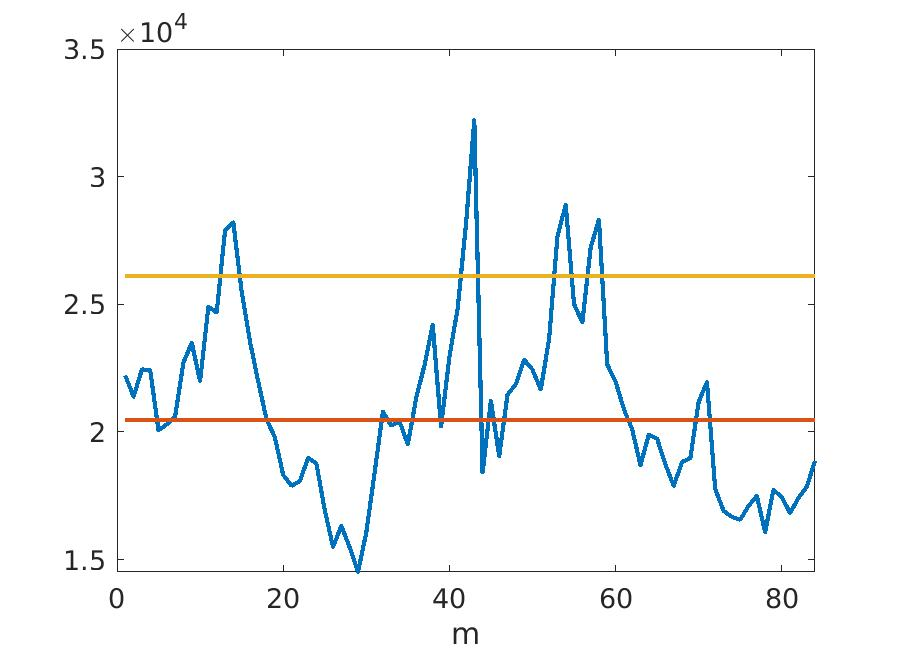
\includegraphics[scale=.12]{../../figs/consecdif_J1_euclid_squared_meandev}(b)\\
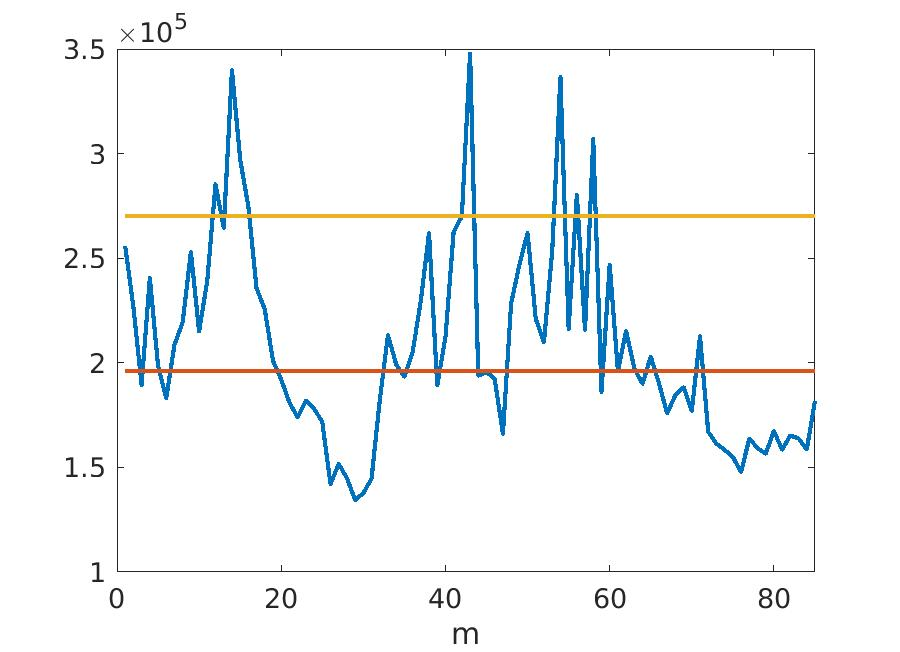
\includegraphics[scale=.12]{../../figs/J2_euclid_squared_meandev}(c)
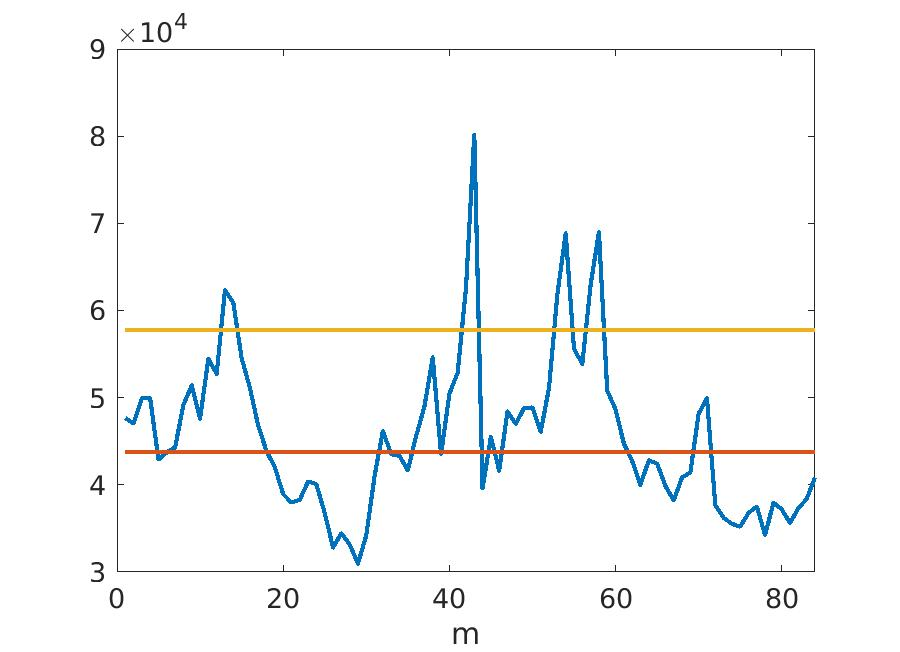
\includegraphics[scale=.12]{../../figs/consecdif_J2_euclid_squared_meandev}(d)\\
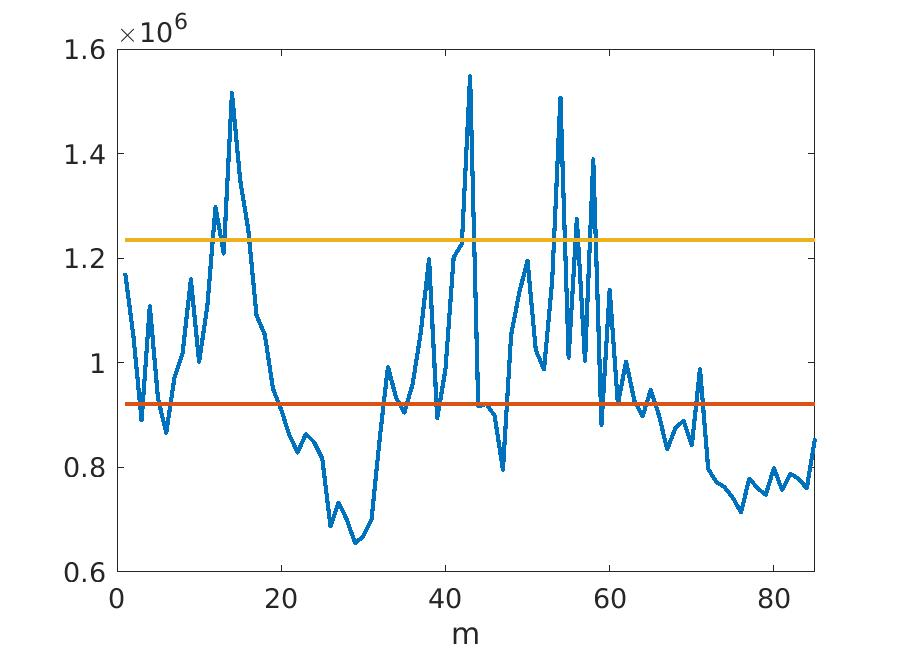
\includegraphics[scale=.12]{../../figs/J3_euclid_squared_meandev}(e)
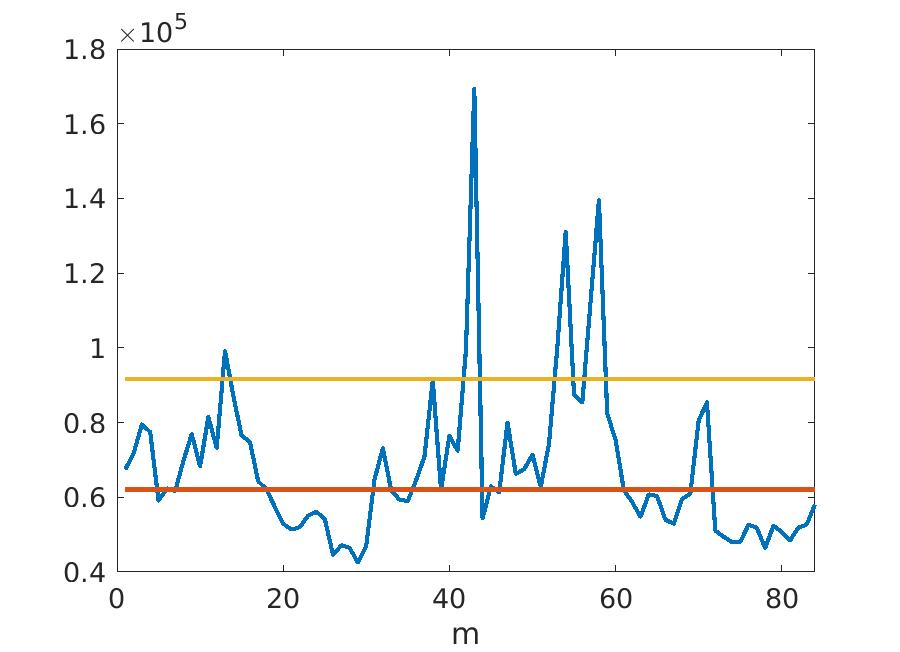
\includegraphics[scale=.12]{../../figs/consecdif_J3_euclid_squared_meandev}(f)\\
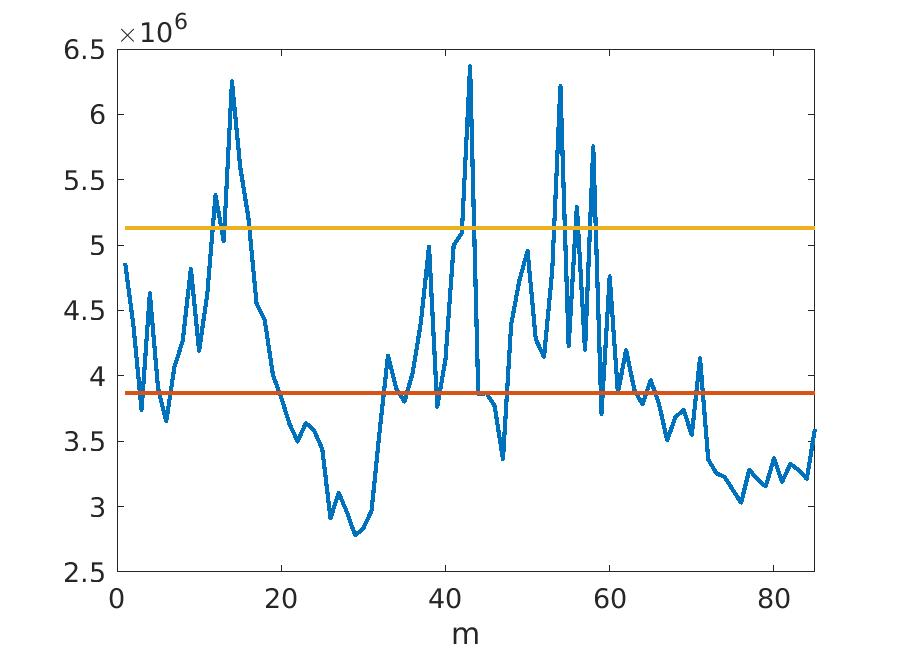
\includegraphics[scale=.12]{../../figs/J4_euclid_squared_meandev}(g)
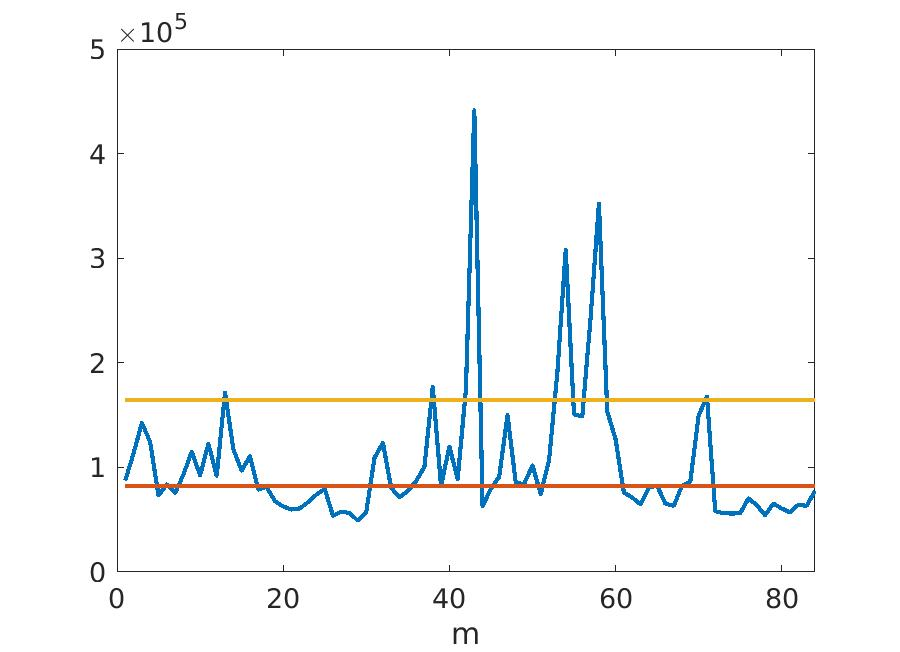
\includegraphics[scale=.12]{../../figs/consecdif_J4_euclid_squared_meandev}(h)
\caption{{\sc Combined Channels} Series of squared deviations $\vd(m)$ and $\vt(m)$. The red horizontal line represents the median value  and the yellow horizontal line represents their median plus two times their absolute median deviation.  $\vd(m)$ - Approximation Levels:  (a) $J=1$; (c) $J=2$; (e) $J=3$; (g) $J=4$. $\vt(m)$ - Approximation Levels:  (b) $J=1$; (d) $J=2$; (f) $J=3$; (h) $J=4$. 
}
\label{F:squared_J1-4_euclid}
\end{figure}


\begin{figure}[htp!]
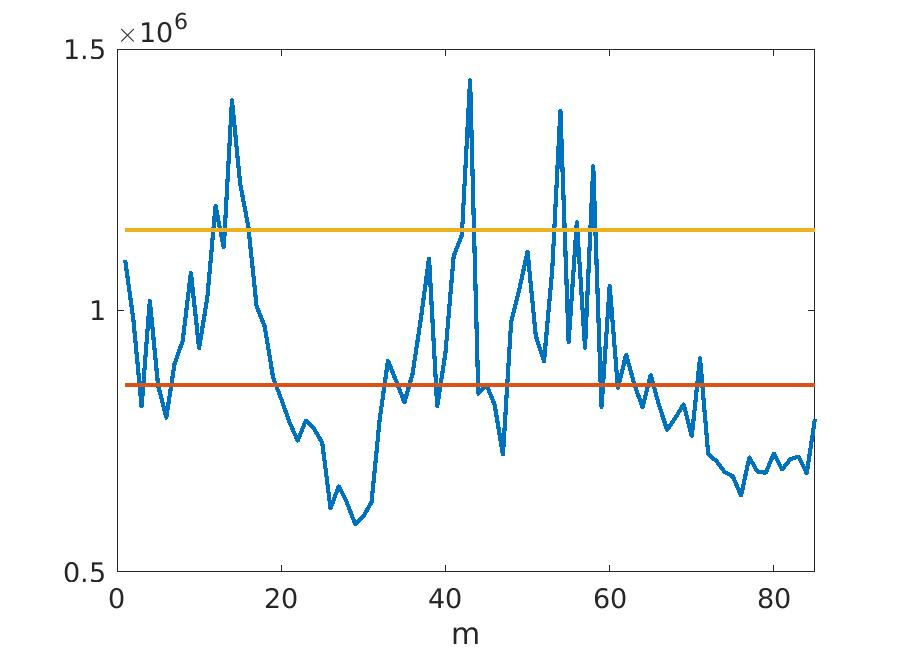
\includegraphics[scale=.12]{../../figs/J3_VV_squared_meandev}(a)
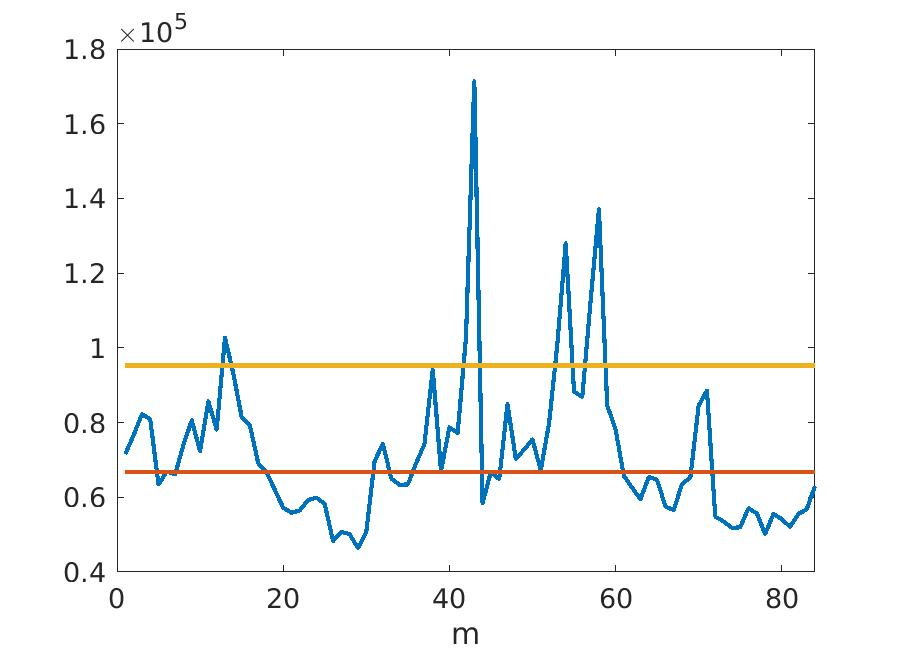
\includegraphics[scale=.12]{../../figs/consecdif_J3_VV_squared_meandev}(b)\\
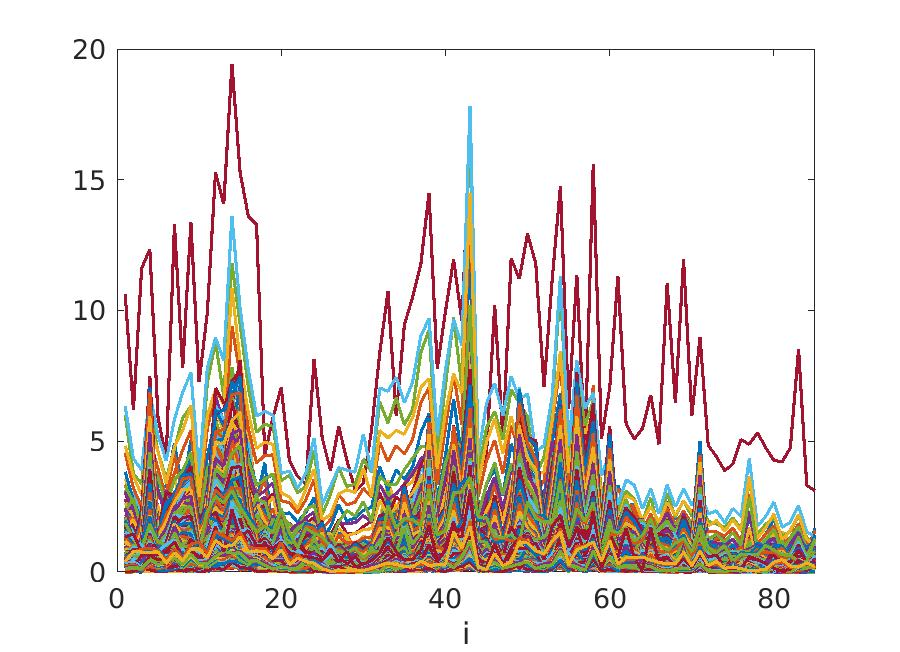
\includegraphics[scale=.12]{../../figs/J3_VV_sqrdif_change_locations}(c)
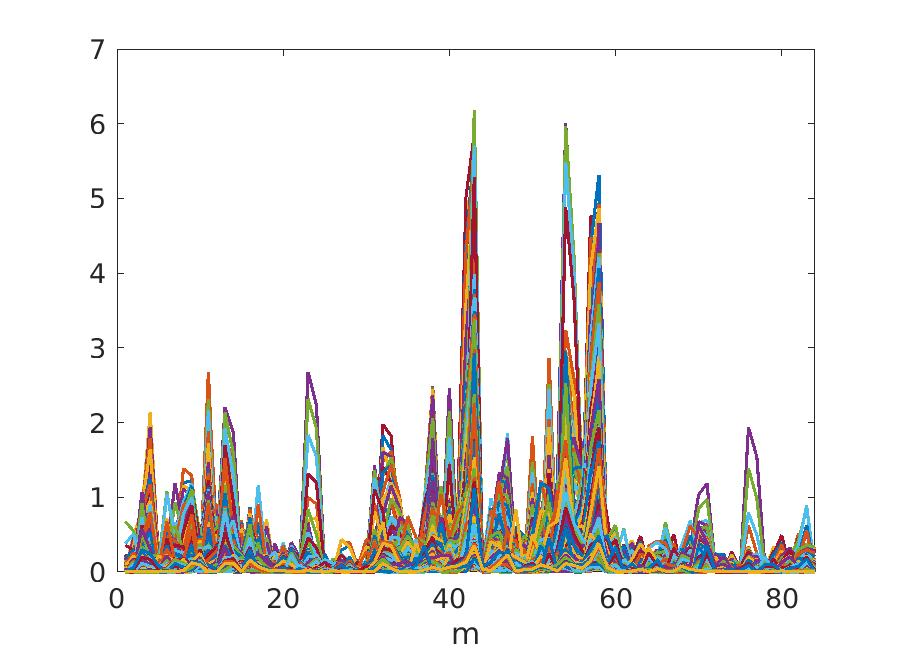
\includegraphics[scale=.12]{../../figs/consecdif_J3_VV_sqrdif_change_locations}(d)\\
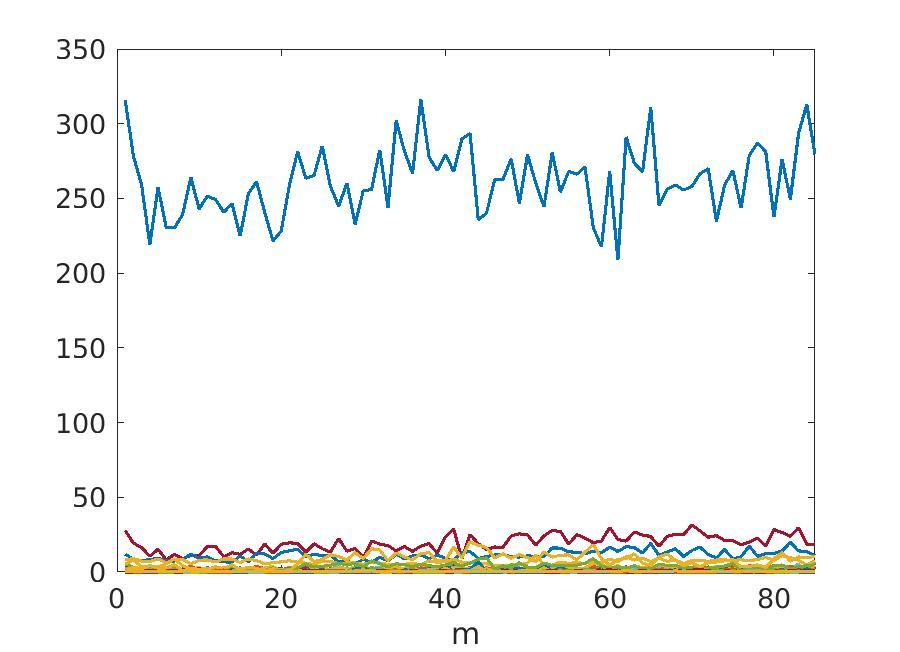
\includegraphics[scale=.12]{../../figs/J3_VV_sqrdif_lowest_cor_locations}(e)
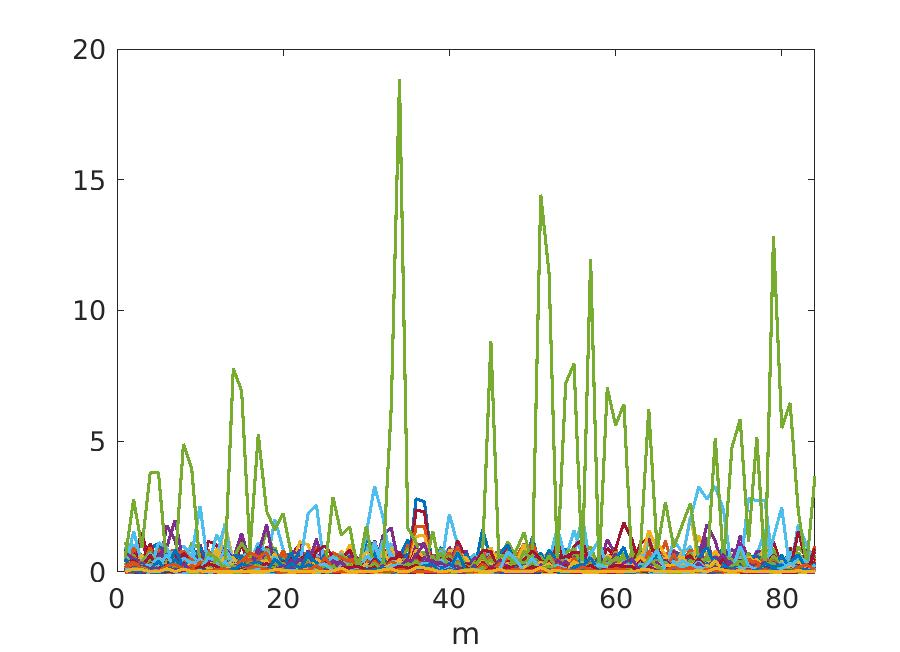
\includegraphics[scale=.12]{../../figs/consecdif_J3_VV_sqrdif_lowest_cor_locations}(f)\\
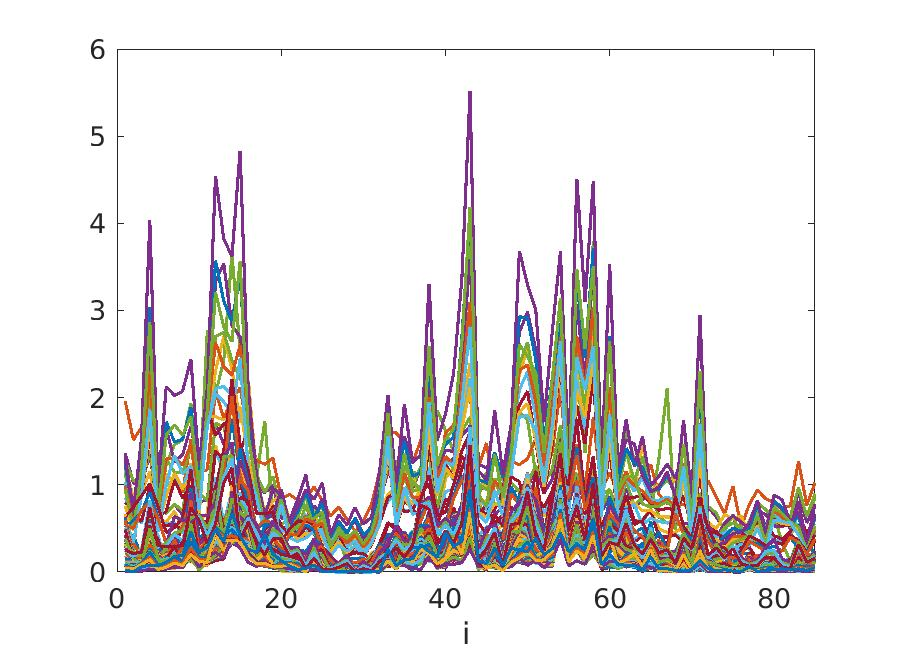
\includegraphics[scale=.12]{../../figs/perc01_J3_VV_sqrdif_change_locations}(g)
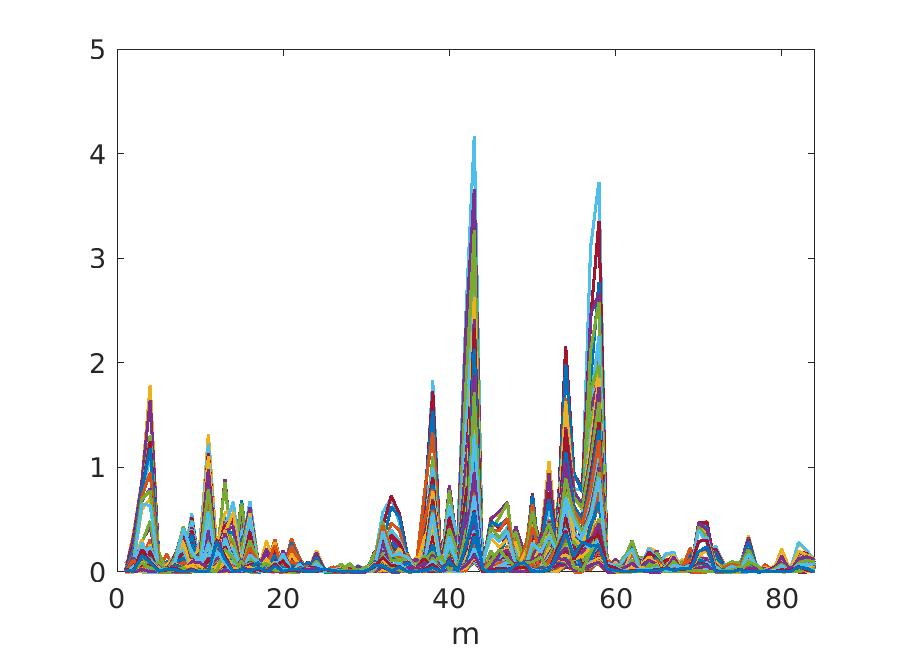
\includegraphics[scale=.12]{../../figs/perc01_consecdif_J3_VV_sqrdif_change_locations}(h)\\
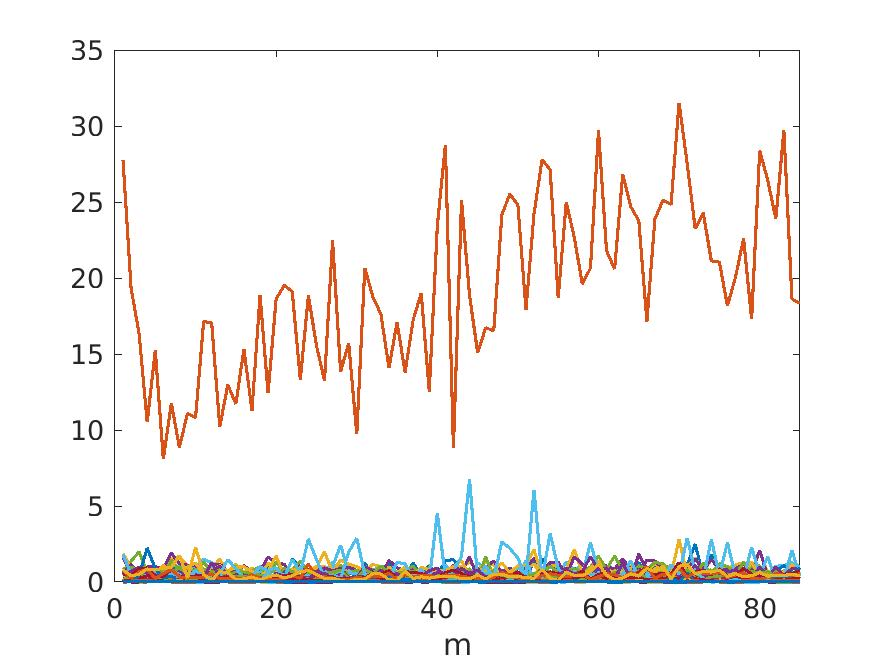
\includegraphics[scale=.12]{../../figs/perc01_J3_VV_sqrdif_lowest_cor_locations}(i)
\includegraphics[scale=.12]{../../figs/perc01_consecdif_J3_VV_sqrdif_lowest_cor_locations}(j)
\caption{{\sc VV Polarization Channel} Series of squared mean deviations at level $J=3$: (a) $\vd(m)$; (b) $\vt(m)$. Red horizontal line represents the median value and yellow line represents two absolute median deviations beyond the median. Squared approximation coefficient deviations: 0.1\% highest absolute correlations - (c) $\vd(m)$;  (d) $\vt(m)$; 0.1\% smallest absolute correlations - (e) $\vd(m)$; (f) $\vt(m)$; 0.01\% highest absolute correlations - (g) $\vd(m)$;  (h) $\vt(m)$;  0.01\% smallest absolute correlations - (i) $\vd(m)$; (j)  $\vt(m)$. 
}  
\label{F:squared_meandev_J3_VV}
\end{figure}

\begin{figure}[htp!]
\includegraphics[scale=.12]{../../figs/J3_VH_squared_meandev}(a)
\includegraphics[scale=.12]{../../figs/consecdif_J3_VH_squared_meandev}(b)

\includegraphics[scale=.12]{../../figs/J3_VH_sqrdif_change_locations}(c)
\includegraphics[scale=.12]{../../figs/consecdif_J3_VH_sqrdif_change_locations}(d)

\includegraphics[scale=.12]{../../figs/J3_VH_sqrdif_lowest_cor_locations}(e)
\includegraphics[scale=.12]{../../figs/consecdif_J3_VH_sqrdif_lowest_cor_locations}(f)

\includegraphics[scale=.12]{../../figs/perc01_J3_VH_sqrdif_change_locations}(g)
\includegraphics[scale=.12]{../../figs/perc01_consecdif_J3_VH_sqrdif_change_locations}(h)

\includegraphics[scale=.12]{../../figs/perc01_J3_VH_sqrdif_lowest_cor_locations}(i)
\includegraphics[scale=.12]{../../figs/perc01_consecdif_J3_VH_sqrdif_lowest_cor_locations}(j)

\caption{{\sc VH Polarization Channel} Series of squared mean deviations at level $J=3$: (a) $\vd(m)$; (b) $\vt(m)$. Red horizontal line represents the median value and yellow line represents two absolute median deviations beyond the median. Squared approximation coefficient deviations: 0.1\% highest absolute correlations - (c) $\vd(m)$;  (d) $\vt(m)$; 0.1\% smallest absolute correlations - (e) $\vd(m)$; (f) $\vt(m)$; 0.01\% highest absolute correlations - (g) $\vd(m)$;  (h) $\vt(m)$;  0.01\% smallest absolute correlations - (i) $\vd(m)$; (j)  $\vt(m)$. 
}  
\label{F:squared_meandev_J3_VH}
\end{figure}

\begin{figure}[htp!]
\includegraphics[scale=.12]{../../figs/J3_euclid_squared_meandev}(a)
\includegraphics[scale=.12]{../../figs/consecdif_J3_euclid_squared_meandev}(b)\\
\includegraphics[scale=.12]{../../figs/J3_euclid_sqrdif_change_locations}(c)
\includegraphics[scale=.12]{../../figs/consecdif_J3_euclid_sqrdif_change_locations}(d)\\
\includegraphics[scale=.12]{../../figs/J3_euclid_sqrdif_lowest_cor_locations}(e)
\includegraphics[scale=.12]{../../figs/consecdif_J3_euclid_sqrdif_lowest_cor_locations}(f)\\
\includegraphics[scale=.12]{../../figs/perc01_J3_euclid_sqrdif_change_locations}(g)
\includegraphics[scale=.12]{../../figs/perc01_consecdif_J3_euclid_sqrdif_change_locations}(h)\\
\includegraphics[scale=.12]{../../figs/perc01_J3_euclid_sqrdif_lowest_cor_locations}(i)
\includegraphics[scale=.12]{../../figs/perc01_consecdif_J3_euclid_sqrdif_lowest_cor_locations}(j)
\caption{{\sc Combined Channels} Series of squared mean deviations at level $J=3$: (a) $\vd(m)$; (b) $\vt(m)$. Red horizontal line represents the median value and yellow line represents two absolute median deviations beyond the median. Squared approximation coefficient deviations: 0.1\% highest absolute correlations - (c) $\vd(m)$;  (d) $\vt(m)$; 0.1\% smallest absolute correlations - (e) $\vd(m)$; (f) $\vt(m)$; 0.01\% highest absolute correlations - (g) $\vd(m)$;  (h) $\vt(m)$;  0.01\% smallest absolute correlations - (i) $\vd(m)$; (j)  $\vt(m)$. 
} 
\label{F:squared_meandev_J3_euclid}
\end{figure}

Figures \ref{F:squared_meandev_J3_VV}-\ref{F:squared_meandev_J3_euclid} present a timewise comparison between overall energy variations, $\vd(m)$ and $\vt(m)$ and their respective individual coefficients. Each figure has ten panels. Panels on the left and right deal with the first and second change detection methods respectively. A full description is give in each figure's caption. The overall conclusion from these figures is that as expected there are temporal variations between the methods regarding change detection (Panels (a)-(b)). The correlation screening detects the most relevant indices, as well as the least relevant ones  (Panels (c)-(f)). 
These conclusions hold for analyses based upon VV, VH or combined polarizations, but the VV polarization signal is much stronger than VH's. A slight advantage is perceived for the $\vd(m)$ method as opposed to $\vt(m)$'s. This makes sense, since we are dealing here with data from a forest region over a long time, and seasonal changes will be perceived more easily on the first proposed method.

\begin{table*}[ht!]
\caption{Absolute correlation thresholds and number of selected coefficients for $n=85$ multi-temporal images of $1200\times 1000$ . Correlation was computed between approximation coefficients and approximation total energy at level $J=2$ for each image. }\label{tabela_quantis}
\centering
\begin{tabular}{c|cccr||c|cccr}
\hline
Qtile &\multicolumn{4}{c||}{\sc Correlation Thresh} &Qtile & \multicolumn{4}{c}{\sc Correlation Thresh}  \\
Level &VV&VH&Comb& Coeffs &Level &VV&VH&Comb& Coeffs \\
\hline
0.50&0.281&0.199&0.292&600000&0.99&0.647&0.582&0.668&12000\\
0.55&0.300&0.218&0.311&540000&0.991&0.651&0.587&0.673&10800\\
0.60&0.319&0.239&0.331&480000& 0.992&0.656&0.594&0.678&9600\\
0.65&0.339&0.260&0.352&420000& 0.993&0.662&0.601&0.684&8400\\
0.70&0.361&0.282&0.375&360000& 0.994&0.669&0.608&0.690&7200\\
0.75&0.385&0.307&0.399&300000& 0.995&0.676&0.617&0.697&6000\\
0.80&0.412&0.335&0.428&240000& 0.996&0.685&0.626&0.705&4800\\
0.85&0.445&0.368&0.462&180000& 0.997&0.696&0.639&0.716&3600\\
0.90&0.487&0.410&0.506&120000& 0.998&0.710&0.654&0.729&2400\\
0.95&0.549&0.472&0.570&60000& 0.999&0.731&0.676&0.748&1200\\
\hline
\end{tabular}
\end{table*}


\begin{figure}[htp!]
\includegraphics[scale=.12]{../../figs/J2_VV_image_cor}(a)
\includegraphics[scale=.12]{../../figs/J2_VH_image_cor}(b)\\
\includegraphics[scale=.12]{../../figs/J2_euclid_image_cor}(c)
\includegraphics[scale=.12]{../../figs/J3_VV_image_cor}(d)\\ 
\includegraphics[scale=.12]{../../figs/J3_VH_image_cor}(e)
\includegraphics[scale=.12]{../../figs/J3_euclid_image_cor}(f)

\caption{Absolute correlation matrices $\vR^{(d)}$ between mean-corrected squared coefficients at approximation levels and overall mean-corrected total energy $\{\vd(m)\}$.  $J=2$ (a)-(c);  $J=3$ (d)-(f). $n=85$ multi-temporal images of $1200\times 1000$ ($J=10$). The color bar on the right gives the magnitude of correlation at all positions. (a) {\sc VV  Polarization - Channel} $J=2$. (b) {\sc VH  Polarization - Channel} $J=2$. (c) {\sc Combined Channels} $J=2$.  (d)  {\sc VV  Polarization - Channel} $J=3$. (e) {\sc VH  Polarization - Channel} $J=3$. (f) {\sc Combined Channels} $J=3$} 
\label{F:image_corr_J2J3}
\end{figure}

\begin{figure}[htp!]
\includegraphics[scale=.12]{../../figs/consecdif_J2_VV_image_cor}(a)
\includegraphics[scale=.12]{../../figs/consecdif_J2_VH_image_cor}(b)\\
\includegraphics[scale=.12]{../../figs/consecdif_J2_euclid_image_cor}(c)
\includegraphics[scale=.12]{../../figs/consecdif_J3_VV_image_cor}(d)\\ 
\includegraphics[scale=.12]{../../figs/consecdif_J3_VH_image_cor}(e)
\includegraphics[scale=.12]{../../figs/consecdif_J3_euclid_image_cor}(f)

\caption{Absolute correlation matrices $\vR^{(t)}$ between squared differences of consecutive log-images' coefficients at approximation levels and their overall total energy $\{\vt(m)\}$. Levels $J=2$ (a)-(c);  $J=3$ (d)-(f). $n=85$ multi-temporal images of $1200\times 1000$. The color bar on the right gives the magnitude of correlation at all positions. (a) {\sc VV  Polarization - Channel} $J=2$. (b) {\sc VH  Polarization - Channel} $J=2$. (c) {\sc Combined Channels} $J=2$. (d)  {\sc VV  Polarization - Channel} $J=3$. (e) {\sc VH  Polarization - Channel} $J=3$. (f) {\sc Combined Channels} $J=3$.} 
\label{F:image_corr_J2J3_consec}
\end{figure}

Figures \ref{F:image_corr_J2J3}-\ref{F:image_corr_J2J3_consec} shows the absolute correlation images for the VV, VH and combined channels for levels $J=2$ and $J=3$. We can notice that high correlation coefficients for $J=2$ are high correlation coefficients for $J=3$ as well. Moreover, there is a clear spatial connection between polarizations and between $\vd(m)$- and $\vt(m)$-based  analyses. On the other hand, correlations are more efficiently segregated when we move: from $J=2$ to $J=3$; from VH to VV polarization; or from  $\vt(m)$ to $\vd(m)$.




\section{Discussion}\label{section_discussion}

We present a novel way of detecting changes in multi-temporal satellite images, WECS. The procedure is based on wavelet energies from both the estimated individual coefficients as well as the whole image approximation. It makes use of correlation screening for ultra-high dimensional data. The proposed method's performance is shown using both synthetic and real data. The proposed method yields spatio-temporal  change points. Its performance is similar to a deep-learning feature extraction method, but the computational cost of the proposed method is 180 times smaller than the cost for the latter. Therefore, we may say that WECS may be used on images with equivalent performance for a fraction of the computational cost. Because of its reliance on wavelet representation and correlation screening, it is sparse, very fast and scalable. Finally, it is easily adapted to be updatable, so that real-time change detection is feasible even with a portable computer.




% if have a single appendix:
%\appendix[Proof of the Zonklar Equations]
% or
%\appendix  % for no appendix heading
% do not use \section anymore after \appendix, only \section*
% is possibly needed

% use appendices with more than one appendix
% then use \section to start each appendix
% you must declare a \section before using any
% \subsection or using \label (\appendices by itself
% starts a section numbered zero.)
%

%
%\appendices
%\section{Proof of the First Zonklar Equation}
%Appendix one text goes here.

% you can choose not to have a title for an appendix
% if you want by leaving the argument blank
%\section{}
%Appendix two text goes here.


% use section* for acknowledgment
%\section*{Acknowledgment}



% Can use something like this to put references on a page
% by themselves when using endfloat and the captionsoff option.
\ifCLASSOPTIONcaptionsoff
  \newpage
\fi



% trigger a \newpage just before the given reference
% number - used to balance the columns on the last page
% adjust value as needed - may need to be readjusted if
% the document is modified later
%\IEEEtriggeratref{8}
% The "triggered" command can be changed if desired:
%\IEEEtriggercmd{\enlargethispage{-5in}}

% references section

% can use a bibliography generated by BibTeX as a .bbl file
% BibTeX documentation can be easily obtained at:
% http://mirror.ctan.org/biblio/bibtex/contrib/doc/
% The IEEEtran BibTeX style support page is at:
% http://www.michaelshell.org/tex/ieeetran/bibtex/
\bibliographystyle{IEEEtran}
% argument is your BibTeX string definitions and bibliography database(s)
\bibliography{bibfile}
%
%% <OR> manually copy in the resultant .bbl file
%% set second argument of \begin to the number of references
%% (used to reserve space for the reference number labels box)
%\begin{thebibliography}{1}
%
%\bibitem{IEEEhowto:kopka}
%H.~Kopka and P.~W. Daly, \emph{A Guide to \LaTeX}, 3rd~ed.\hskip 1em plus
%  0.5em minus 0.4em\relax Harlow, England: Addison-Wesley, 1999.
%
%\end{thebibliography}

% biography section
% 
% If you have an EPS/PDF photo (graphicx package needed) extra braces are
% needed around the contents of the optional argument to biography to prevent
% the LaTeX parser from getting confused when it sees the complicated
% \includegraphics command within an optional argument. (You could create
% your own custom macro containing the \includegraphics command to make things
% simpler here.)
%\begin{IEEEbiography}[{\includegraphics[width=1in,height=1.25in,clip,keepaspectratio]{mshell}}]{Michael Shell}
% or if you just want to reserve a space for a photo:


%\begin{IEEEbiography}
%[{\includegraphics[width=1in,height=1.25in,clip,keepaspectratio]{../Photo/rodney}}]{Rodney Fonseca}
%was born in Brazil, in 1993. He received the Master’s
%degrees in Statistics from the Federal University of Pernambuco,
%Recife, Brazil, in 2017, and the Ph.D. degree in Statistics, from Campinas State University, Campinas, Brazil, in 2021.
%His research interests include nonparametric statistics, time series, graph signal processing and regression models.
%\end{IEEEbiography}
%\vfill
%
%\begin{IEEEbiography}[{\includegraphics[width=1in,height=1.25in,clip,keepaspectratio]{../Photo/aluisio}}]{Alu\'{i}sio~Pinheiro}
%was born in Brazil, in 1967. He received the Master’s degree in Statistics from Campinas State University, Campinas, Brazil, in 1992, and the Ph.D. degree in Statistics from University of North Carolina, Chapel Hill, US, in 1997.
%He is currently Professor at Campinas State University. His research interests concern U-statistics, wavelets, nonparametric statistics and time series.
%Dr. Pinheiro was the 2012 Pranab Kumar Sen Distinguished Visiting Professor of Biostatistics, UNC-Chapel Hill. He has been the Brazilian Statistics Association General Secretary (2010-2012) and Treasurer (2018-2020).
%\end{IEEEbiography}
%
%
%\begin{IEEEbiography}[{\includegraphics[width=1in,height=1.25in,clip,keepaspectratio]{../Photo/abdou}}]{Abdourrahmane Mahamane Atto}
%was born in Niger, in 1974. He received the Master’s
%degrees in applied mathematics and pure mathematics from the University of Abomey-Calavi,
%Cotonou, Benin, 2001 and 2002, respectively, the
%Master’s degree of advanced studies in electrical engineering from the École Polytechnique d’Abomey-Calavi, Cotonou, in 2002, and the Ph.D. degree
%in applied mathematics, codelivered by TELECOM
%Bretagne, Brest, France, and the University of
%Rennes I, Rennes, France, in 2008.
%He worked with École Polytechnique d’Abomey-Calavi, from 2002 to 2003,
%Ecole des Mines, de l’Industrie et de la Géologie, Niamey, Niger, from 2003
%to 2004, TELECOM Bretagne, from 2008 to 2009, and Institut Polytechnique
%de Bordeaux, Talence, France, from 2009 to 2011. Since September 2011, he
%has been an Associate Professor at the University of Savoie, Polytech Annecy-Chambéry, Annecy, France. His research interests concern mathematical methods and models for signal, image, and information processing.
%\end{IEEEbiography}
%\vfill

% You can push biographies down or up by placing
% a \vfill before or after them. The appropriate
% use of \vfill depends on what kind of text is
% on the last page and whether or not the columns
% are being equalized.

%\vfill

% Can be used to pull up biographies so that the bottom of the last one
% is flush with the other column.
%\enlargethispage{-5in}



% that's all folks
\end{document}


